\chapter{Studi Literatur}

\section{Qubit}
\par
Dalam sistem komputasi klasik, bit merupakan satuan informasi paling dasar yang hanya dapat memiliki dua keadaan diskrit, yaitu 0 atau 1 \cite{nielsen2010quantum}. Setiap operasi logika dalam komputer klasik dibangun dari manipulasi terhadap bit-bit ini, yang secara fisik dapat direpresentasikan oleh dua kondisi berbeda, seperti arus listrik yang mengalir atau tidak mengalir, tegangan tinggi atau rendah, serta keadaan magnetik utara atau selatan \cite{tanenbaum2013structured}. Dengan demikian, bit berfungsi sebagai pembawa informasi biner yang menjadi fondasi bagi seluruh proses komputasi konvensional \cite{shannon1948mathematical}.
\par
Namun, seiring berkembangnya pemahaman terhadap prinsip-prinsip mekanika kuantum, muncul paradigma baru dalam penyimpanan dan pemrosesan informasi yang dikenal sebagai qubit (quantum bit) \cite{nielsen2010quantum}. Tidak seperti bit klasik yang hanya dapat berada dalam satu keadaan tertentu pada satu waktu, qubit mampu berada dalam superposisi antara keadaan $\ket{0}$ dan $\ket{1}$ secara bersamaan \cite{dirac1981principles}. Transisi dari bit ke qubit ini menandai pergeseran fundamental dari logika deterministik menuju logika probabilistik-kuantum, di mana informasi tidak lagi direpresentasikan secara biner murni, melainkan sebagai vektor dalam ruang Hilbert dua dimensi yang memiliki representasi matriks sebagai berikut \cite{sakurai2017modern}.

\begin{equation}
	\ket{0} = \begin{pmatrix} 1 \\ 0 \end{pmatrix}
\end{equation}
dan
\begin{equation}
	\ket{1} = \begin{pmatrix} 0 \\ 1 \end{pmatrix}
\end{equation}
\par
Kombinasi linier dari dua qubit atau basis vektor yang menyatakan keadaan informasi kuantum secara umum dituliskan menjadi
\begin{equation}
	\ket{\psi} = \alpha \ket{0} + \beta \ket{1}\label{keadaanumum}
\end{equation}
dengan $\alpha$ dan $\beta$ adalah bilangan kompleks. Keadaan tersebut harus memenuhi syarat normalisasi atau $\langle \psi | \psi \rangle = 1$. Sehingga $\alpha$ dan $\beta$ harus memenuhi
\begin{equation}
	|\alpha|^2 + |\beta|^2 = 1
\end{equation}

\par
Sistem yang terdiri atas lebih dari satu qubit maka keadaan sistemnya dapat dinyatakan dengan perkalian langsung dari masing-masing keadaannya \cite{mermin2007quantum, bengtsson2017geometry, barnett2009quantum, schlosshauer2007decoherence}. Misalkan informasi yang dimiliki yaitu bilangan 2 dan 6 yang apabila dinyatakan dalam bit klasik akan menjadi 10 dan 110. Informasi tersebut jika dinyatakan secara kuantum maka dapat dituliskan menjadi
\begin{equation}
	10 \rightarrow \ket{1} \otimes \ket{0}
\end{equation}
dan
\begin{equation}
	110 \rightarrow \ket{1} \otimes \ket{1} \otimes \ket{0}
\end{equation}
atau secara ringkas juga dapat dituliskan menjadi
\begin{equation}
	\ket{1} \otimes \ket{0} = \ket{10}
\end{equation}
dan
\begin{equation}
	\ket{1} \otimes \ket{1} \otimes \ket{0} = \ket{110}
\end{equation}
\par

Qubit juga memiliki realitas fisis, beberapa diantaranya adalah pada kasus polarisasi foton \cite{nielsen2010quantum}. Pada polarisasi, $\ket{0}$ merupakan representasi dari polarisasi vertikal foton, sedangkan $\ket{1}$ untuk polarisasi horizontalnya \cite{kok2007linear}. Qubit juga dapat digunakan menjadi representasi dari spin elektron, misalnya $\ket{0}$ adalah representasi dari spin-up dan $\ket{1}$ sebagai spin-down \cite{sakurai2017modern}.

\subsection{Representasi Bola Bloch}
\par
Suatu keadaan qubit dapat direpresentasikan dalam bola Bloch. Dengan mengambil bentuk polar pada koefisien dalam persamaan (\ref{keadaanumum}), yaitu $\alpha = |\alpha| e^{i\varphi_\alpha}$ dan $\beta = |\beta| e^{i\varphi_\beta}$, maka persamaan (\ref{keadaanumum}) dapat dituliskan sebagai
\begin{equation}\label{kk}
	\ket{\psi}=|\alpha| e^{i\varphi_\alpha}\ket{0}+|\beta| e^{i\varphi_\beta}\ket{1}.
\end{equation}
Karena $|\alpha|^2 + |\beta|^2 = 1$, maka koefisien tersebut dapat diparameterisasi sebagai
\begin{equation}
	|\alpha|=\cos \theta, \ |\beta|=\sin \theta,
\end{equation}
dengan $\cos\theta$ dan $\sin\theta$ bernilai positif sehingga parameter $\theta$ dibatasi pada rentang $0 \leq \theta \leq \frac{\pi}{2}$ \cite{Blumel}.
\par
Selanjutnya, persamaan (\ref{kk}) dapat dituliskan sebagai
\begin{equation}
	\begin{aligned}
		\ket{\psi} &= \cos \theta \, e^{i\varphi_\alpha} \ket{0} + \sin \theta \, e^{i\varphi_\beta} \ket{1} \\
		&= e^{i\varphi_\alpha} \left( \cos \theta \ket{0} + \sin \theta \, e^{i(\varphi_\beta - \varphi_\alpha)} \ket{1} \right).
	\end{aligned}
\end{equation}
Faktor global $e^{i\varphi_\alpha}$ dapat diabaikan karena tidak bersifat observabel. Dengan mendefinisikan $\varphi = \varphi_\beta - \varphi_\alpha$, persamaan di atas menjadi
\begin{equation}\label{poin}
	\ket{\psi} = \cos\theta \ket{0} + \sin\theta \, e^{i\varphi} \ket{1}.
\end{equation}
Jika dilakukan substitusi $\theta \Rightarrow \frac{\theta}{2}$, maka persamaan di atas dapat dituliskan sebagai
\begin{equation}\label{bloch}
	\ket{\psi} = \cos \frac{\theta}{2} \ket{0} + \sin \frac{\theta}{2} \, e^{i\varphi} \ket{1}.
\end{equation}
Persamaan tersebut merepresentasikan keadaan qubit dalam bola Bloch, seperti ditunjukkan pada Gambar~(\ref{fig:Blochsphere}), dengan batasan $0 \leq \theta \leq \pi$ dan $0 \leq \varphi \leq 2\pi$.
\begin{figure}[htbp]
	\centering
	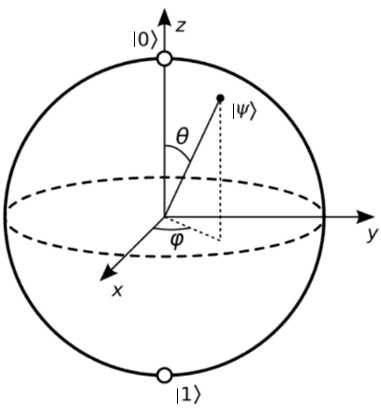
\includegraphics[width=0.6\textwidth]{Bloch_Sphere} % sesuaikan path dan ukuran gambar
	\caption{Bola Bloch}
	\label{fig:Blochsphere}
	\cite{Meoijuan}
\end{figure}

Keadaan qubit dapat direpresentasikan sebagai titik-titik pada permukaan bola Bloch \cite{preskill_notes,Desurvire2009}. Titik-titik tersebut dapat dinyatakan dalam koordinat Kartesian ($x$, $y$, $z$), dengan
\begin{equation}
	\begin{aligned}
		x &= \sin\theta \cos\varphi, \\
		y &= \sin\theta \sin\varphi, \\
		z &= \cos\theta.
	\end{aligned}
\end{equation}
Dengan demikian, vektor pada bola Bloch dapat dituliskan sebagai \cite{pathak2013elements}
\begin{equation}\label{nn}
	\begin{aligned}
		\hat{n} &= x \, \hat{i} + y \, \hat{j} + z \, \hat{k} \\
		&= \sin\theta \cos\varphi \, \hat{i} + \sin\theta \sin\varphi \, \hat{j} + \cos\theta \, \hat{k}.
	\end{aligned}
\end{equation}

\subsection{Keadaan Dua Qubit}
Keadaan umum untuk dua qubit adalah
\begin{equation}
	\ket{\psi}=c_{00}\ket{00}+c_{01}\ket{01}+c_{10}\ket{10}+c_{11}\ket{11} \label{2.16}
\end{equation}
atau
\begin{equation}
	\ket{\psi}=\sum_{i,j=0}^{1} c_{ij} \ket{ij}\label{umum2qubit}
\end{equation}
dengan koefisien kompleks yang memenuhi
\begin{equation}
	|c_{00}|^2+|c_{01}|^2+|c_{10}|^2+|c_{11}|^2=1
\end{equation}

Contoh 1.
\begin{equation}
	\ket{\psi_1}=\frac{1}{2}(\ket{00}+\ket{01}+\ket{10}+\ket{11}) \label{contoh1}
\end{equation}
dengan $c_{00}=c_{01}=c_{10}=c_{11}=\frac{1}{2}$.

Contoh 2.
\begin{equation}
	\ket{\psi_2}=\frac{1}{2}(\ket{00}+\ket{01}+\ket{10}-\ket{11})\label{contohkeadaan2qubit}
\end{equation}
dengan $c_{00}=c_{01}=c_{10}=-c_{11}=\frac{1}{2}$.

Contoh 3.
\begin{equation}
	\ket{\psi_3}=\frac{1}{2}(\ket{00}+\ket{01}-\ket{10}-\ket{11}) \label{contoh3}
\end{equation}
dengan $c_{00}=c_{01}=-c_{10}=-c_{11}=\frac{1}{2}$.

Contoh 4.
\begin{equation}
	\ket{\psi_4}=0,1\ket{00}+0,5\ket{01}+0,5\ket{10}+0,7\ket{11} \label{contoh4}
\end{equation}
dengan $c_{00}=0,1, c_{01}=c_{10}=0,5, c_{11}=0,7$.

Contoh 5.
\begin{equation}
	\ket{\psi_5}=\frac{1}{\sqrt{2}}(\ket{00}+\ket{11}) \label{contoh5}
\end{equation}
dengan $c_{00}=c_{11}=\frac{1}{\sqrt{2}}$ dan $c_{01}=c_{10}=0$.

\subsection{Keadaan Tiga Qubit}
Keadaan umum untuk tiga qubit adalah
\begin{equation}
	|\psi_{ABC}\rangle = \sum_{i,j,k=0}^{1}c_{ijk} |ijk|\label{keadaan3qubit}
\end{equation}
\begin{equation*}
	=c_{000} |000\rangle
	+ c_{001} |001\rangle
	+ c_{010} |010\rangle
	+ c_{011} |011\rangle
\end{equation*}
\begin{equation*}
	+ c_{100} |100\rangle
	+ c_{101} |101\rangle
	+ c_{110} |110\rangle
	+ c_{111} |111\rangle ,
\end{equation*}
dengan syarat normalisasi
\begin{equation}
	\sum_{i,j,k=0}^{1} |c_{ijk}|^2 = |c_{000}|^2 + |c_{001}|^2 + \cdots + |c_{110}|^2 + |c_{111}|^2 = 1.\label{normalisasi3qubit}
\end{equation}

Contoh 6.
\begin{equation}
	|\psi_6\rangle =
	\frac{1}{2}
	\left(
	|000\rangle + |001\rangle + |010\rangle + |011\rangle
	\right)\label{contohkeadaan3qubit}
\end{equation}
dengan $c_{000}=c_{001}=c_{010}=c_{011}=\frac{1}{2}$ dan $c_{100}=c_{101}=c_{110}=c_{111}=0$.

Contoh 7.
\begin{equation}
	\ket{\psi_7}=\frac{1}{\sqrt{2}}(\ket{000}+\ket{111})\label{contohkeadaan3qubitkedua}
\end{equation}
dengan $c_{000}=c_{111}=\frac{1}{\sqrt{2}}$ dan $c_{001}=c_{010}=c_{110}=c_{100}=c_{101}=c_{110}=0$.

Contoh 8.
\begin{equation}
	\ket{\psi_8}=\frac{1}{\sqrt{3}}(\ket{001}+\ket{010}+\ket{100})\label{contohkeadaan3qubitketiga}
\end{equation}
dengan $c_{001}=c_{010}=c_{100}=\frac{1}{\sqrt{3}}$ dan koefisien yang lainnya bernilai 0.

\subsection{Keadaan n-Qubit}
\par
Sistem kuantum yang terdiri atas lebih dari satu qubit merupakan fondasi utama dalam teori informasi kuantum, komputasi kuantum, serta kajian keterikatan kuantum multipartit. Secara matematis, keadaan sistem kuantum multipartit direpresentasikan dalam ruang Hilbert hasil kali tensor dari ruang Hilbert masing-masing subsistem \cite{nielsen2010quantum}. Generalisasi konsep ini pada sistem dengan $n$ qubit menghasilkan struktur ruang keadaan yang jauh lebih kompleks, dengan dimensi ruang Hilbert sebesar $2^n$ \cite{preskill_lecture_notes}. Secara umum kombinasi linier untuk sistem dengan keadaan n qubit dapat dituliskan sebagai berikut
\begin{equation}
	\ket{\psi}=c_{00...0}\ket{00...0}+c_{00...01}\ket{00...01}+...+c_{11...1}\ket{11...1}
\end{equation}
atau
\begin{equation}
	\ket{\psi}=\sum_{i_1,i_2,...,i_n}^1 c_{i_1 i_2...i_n}\ket{i_1 i_2...i_n}
\end{equation}
dengan
\begin{equation}
	\sum_{i_1,i_2,...,i_n=0}^{1}|c_{i_1 i_2...i_n}|^2=1
\end{equation}

Keadaan n-qubit yang dapat dituliskan sebagai hasil kali tensor dari keadaan masing-masing qubit disebut sebagai keadaan terpisah \cite{Werner1989,bengtsson2017geometry}. Sebaliknya, apabila keadaan tersebut tidak dapat direpresentasikan dalam bentuk hasil kali tensor sederhana, maka keadaan tersebut tergolong sebagai keadaan terikat (entangled state) \cite{horodecki2009quantum}. Fenomena keterikatan kuantum ini menjadi ciri khas utama mekanika kuantum dan memainkan peran penting dalam berbagai aplikasi kuantum modern, termasuk teleportasi kuantum, kriptografi kuantum, dan komputasi kuantum \cite{bennett_1993}.

\section{Keterbelitan}
\subsection{Keterbelitan Keadaan Dua Qubit}
\par
Suatu keadaan (2.16) dikatakan terpisah jika dan hanya jika memenuhi
\begin{equation}
	\ket{\psi_1}\otimes\ket{\psi_2}.
\end{equation}
Sebaliknya, jika tidak memenuhi bentuk di atas maka dikatakan keadaan terbelit (\textit{entangled}) \cite{esteve2004quantum}.

\subsubsection{Keadaan Terpisah}
Misalkan $\ket{\psi_1}$ dan $\ket{\psi_2}$ dalam keadaan dua qubit sebagai berikut
\begin{equation}
	\ket{\psi_1}=x_0\ket{0}+x_1\ket{1}\\
	\ket{\psi_2}=y_0\ket{0}+y_1\ket{1}\label{2.34}
\end{equation}
dan suatu keadaan dua qubit yang belum diketahui keterbelitannya sebagaimana persamaan (2.16), maka
\begin{equation*}
	\ket{\psi}=\ket{\psi_1}\otimes\ket{\psi_2}
\end{equation*}
\begin{equation*}
	=(x_0\ket{0}+x_1\ket{1})\otimes(y_0\ket{0}+y_1\ket{1})
\end{equation*}
\begin{equation}
	=x_0y_0\ket{00}+x_0y_1\ket{01}+x_1y_0\ket{10}+x_1y_1\ket{11}
\end{equation}
di mana
\begin{equation*}
	c_{00}=x_0y_0
	\label{eq:terbelit1}
\end{equation*}
\begin{equation*}
	c_{01}=x_0y_1
	\label{eq:terbelit2}
\end{equation*}
\begin{equation*}
	c_{10}=x_1y_0
	\label{eq:terbelit3}
\end{equation*}
\begin{equation}
	c_{11}=x_1y_1
	\label{eq:terbelit4}
\end{equation}
Jika koefisien $c_{00}$, $c_{01}$, $c_{10}$, dan $c_{11}$ berturut-turut bisa diuraikan dalam perkalian $x_0y_0$, $x_0y_1$, $x_1y_0$, dan $x_1y_1$, maka keadaan dikatakan terpisah \cite{taufiqi2024asymmetric}. Keadaan (\ref{contoh1}) adalah keadaan terpisah, karena $x_0=x_1=\frac{1}{\sqrt{2}}$ dan $y_0=y_1=\frac{1}{\sqrt{2}}$. Keadaan (\ref{contoh3}) juga keadaan terpisah karena dapat diperoleh $x_0=-x_1=\frac{1}{\sqrt{2}}$ dan $x_0=x_1=\frac{1}{\sqrt{2}}$.

\subsubsection{Keadaan Terbelit}
Keadaan-keadaan pada contoh 2 (\ref{contohkeadaan2qubit}), contoh 4 (\ref{contoh4}), dan contoh 5 (\ref{contoh5}) adalah keadaan terbelit karena kita tidak dapat menemukan nilai dari $x_0$, $x_1$, $y_0$, dan $y_1$ secara pasti.

\subsection{Keterbelitan Keadaan Tiga Qubit}
Ditinjau keadaan tiga qubit secara umum seperti pada persamaan (\ref{keadaan3qubit}) dengan syarat normalisasi seperti pada persamaan (\ref{normalisasi3qubit}). Keadaan tiga qubit mempunyai sifat yang lebih rumit dari keadaan dua qubit. Sifat yang dimiliki selain terpisah sempurna dan terbelit sempurna sebagaimana keadaan dua qubit, juga memiliki sifat terbelit sebagian \cite{Acin2001,Seevinck2008,Verstraete2002}.

\subsubsection{Keadaan Terpisah Sempurna}
Seperti halnya keadaan dua qubit secara umum, keadaan tiga qubit ini bisa tersusun atas
tiga keadaan sub-sistem qubit tunggal $|\phi_A\rangle$, $|\phi_B\rangle$, dan $|\phi_C\rangle$
sebagai berikut

\begin{equation*}
	|\psi_A\rangle = x_0 |0\rangle + x_1 |1\rangle
\end{equation*}
\begin{equation}
	|\psi_B\rangle = y_0 |0\rangle + y_1 |1\rangle
\end{equation}
\begin{equation*}
	|\psi_C\rangle = z_0 |0\rangle + z_1 |1\rangle ,
\end{equation*}
dengan syarat normalisasi

\begin{equation}
	\sum_{i=0}^{1} |x_i|^2
	=
	\sum_{j=0}^{1} |y_j|^2
	=
	\sum_{k=0}^{1} |z_k|^2
	= 1 .
\end{equation}

Jika dapat diperoleh $x_0, x_1, y_0, y_1, z_0$, dan $z_1$ maka suatu keadaan disebut terpisah sempurna, di mana

\begin{align}
	c_{000} &= x_0 y_0 z_0 \nonumber \\
	c_{001} &= x_0 y_0 z_1 \nonumber \\
	c_{010} &= x_0 y_1 z_0 \nonumber \\
	c_{011} &= x_0 y_1 z_1 \nonumber \\
	c_{100} &= x_1 y_0 z_0 \nonumber \\
	c_{101} &= x_1 y_0 z_1 \nonumber \\
	c_{110} &= x_1 y_1 z_0 \nonumber \\
	c_{111} &= x_1 y_1 z_1 \label{koefisien3qubit}.
\end{align}
Keadaan (\ref{contohkeadaan3qubit}) pada contoh 6 adalah keadaan terpisah sempurna, karena dapat dinyatakan menjadi

\begin{equation}
	|\chi_1\rangle
	=
	|0\rangle_A \otimes
	\left(
	\frac{1}{\sqrt{2}}
	(|0\rangle + |1\rangle)
	\right)_B
	\otimes
	\left(
	\frac{1}{\sqrt{2}}
	(|0\rangle + |1\rangle)
	\right)_C .
\end{equation}
dengan $x_0=x_1=0$, $y_0=y_1=\frac{1}{\sqrt{2}}=z_0=z_1$.

\subsubsection{Keadaan Terbelit Sempurna}
\par
Jika suatu keadaan tidak dapat diperoleh nilai $x_0, x_1, y_0, y_1, z_0$, dan $z_1$ secara pasti maka keadaan tersebut merupakan keadaan terbelit sempurna. Contoh keadaan terbelit sempurna adalah keadaan yang dituliskan pada persamaan (\ref{contohkeadaan3qubitketiga}).

\subsubsection{Keadaan Terbelit Sebagian}
\par
Selain dua sifat sebelumnya, keadaan tiga qubit juga mempunyai sifat terbelit sebagian, yaitu dua qubit terbelit dan 1 qubit terpisah, dengan pola sebagai berikut.
\begin{equation}
	|\psi\rangle
	=
	|\psi\rangle_{A} \otimes
	|\psi\rangle_{BC},
\end{equation}
\begin{equation}
	|\psi\rangle
	=
	|\psi\rangle_{AB} \otimes
	|\psi\rangle_{C},
\end{equation}
dan qubit pertama dan ketiga terbelit sedangkan qubit kedua terurai. Pola terakhir ini tidak dapat dituliskan sebagai bentuk perkalian seperti di atas.
Contoh 9. Keadaan
\begin{equation}
	|\psi_9\rangle =
	\frac{1}{\sqrt{2}}
	\left(
	|000\rangle + |011\rangle
	\right) ,
\end{equation}
dengan
\begin{equation}
	c_{000}=c_{011}=\frac{1}{\sqrt{2}}
\end{equation}
dan
\begin{equation}
	c_{001}=c_{010}=c_{100}=c_{101}=c_{110}=c_{111}=0
\end{equation}
dapat dituliskan kembali menjadi
\begin{equation}
	|\psi_9\rangle
	=
	|\psi\rangle_{A-BC}
	=
	|0\rangle_A \otimes
	\left(
	\frac{1}{\sqrt{2}}
	(|00\rangle + |11\rangle)
	\right)_{BC} .
\end{equation}
Contoh 10. Keadaan
\begin{equation}
	|\psi_{10}\rangle
	=
	\frac{1}{2}
	\left(
	|001\rangle + |011\rangle + |101\rangle - |111\rangle
	\right) .
\end{equation}
dengan
\begin{equation}
	c_{001}=c_{011}=c_{101}=-c_{111}=\frac{1}{2}
\end{equation}
dan
\begin{equation}
	c_{000}=c_{010}=c_{100}=c_{110}=0
\end{equation}
dapat dituliskan dalam bentuk
\begin{equation}
	|\psi_{10}\rangle
	=
	\left(
	\frac{1}{2}
	(|00\rangle + |01\rangle + |10\rangle - |11\rangle)
	\right)_{AB}
	\otimes
	|1\rangle_C .
\end{equation}
\par
Selain keadaan gabungan $A$-$BC$ (sub-sistem $A$ dan sub-sistem $BC$) dan $AB$-$C$ (sub-sistem $AB$ dan sub-sistem $C$), terdapat satu keadaan gabungan lainnya yaitu keadaan gabungan $AC$-$B$ (sub-sistem $AC$ dan sub-sistem $B$), dengan contoh
keadaannya bisa dituliskan sebagai

\begin{equation}
	|\psi\rangle
	=
	\frac{1}{2}
	\left(
	|000\rangle + |010\rangle + |101\rangle + |111\rangle
	\right) .
\end{equation}
dengan

\begin{equation}
	c_{000}=c_{010}=c_{101}=c_{111}=\frac{1}{2}
\end{equation}
dan

\begin{equation}
	c_{001}=c_{100}=c_{011}=c_{110}=0
\end{equation}
Evaluasi memberikan $y_0=y_1=\frac{1/2}{\sqrt{2}}$, tetapi tidak ada nilai yang konsisten bagi $x_i$ dan $z_i$. Karena itu, keadaan ini terurai menjadi AC-B. Namun, kita tidak bisa menuliskan keadaan $|\psi\rangle$ seperti berikut

\begin{equation}
	|\psi\rangle
	\neq
	\left(
	\frac{1}{\sqrt{2}}
	(|00\rangle + |11\rangle)
	\right)_{AC}
	\otimes
	\left(
	\frac{1}{\sqrt{2}}
	(|0\rangle + |1\rangle)
	\right)_B ,
\end{equation}
karena justru akan menjadi keadaan gabungan $AB$-$C$. Kita juga tidak bisa menuliskan keadaan menjadi

\begin{equation}
	|\psi\rangle
	\neq
	\left(
	\frac{1}{\sqrt{2}}
	(|0\rangle + |1\rangle)
	\right)_B
	\otimes
	\left(
	\frac{1}{\sqrt{2}}
	(|00\rangle + |11\rangle)
	\right)_{AC} ,
\end{equation}
karena justru akan menjadi keadaan gabungan $A$-$BC$.

\section{Kelas Keterbelitan Kuantum Tiga Qubit}
\par
Keterbelitan kuantum merupakan fenomena yang hanya dapat dijelaskan dalam kerangka mekanika kuantum dan menjadi sumber daya utama dalam informasi kuantum dan komputasi kuantum \cite{horodecki2009quantum}. Dalam sistem multipartit, keterbelitan menjadi semakin kompleks karena melibatkan interaksi beberapa partikel secara tidak terpisahkan. Dalam teori informasi kuantum, kelas keterbelitan merupakan pengelompokan keadaan-keadaan kuantum yang memiliki karakteristik keterbelitan yang sama berdasarkan jenis transformasi lokal yang diperbolehkan. Dua keadaan kuantum dikatakan berada dalam satu kelas keterbelitan apabila salah satu keadaan dapat diubah menjadi keadaan lainnya melalui operasi lokal pada masing-masing subsistem dan komunikasi klasik \cite{Bennett1996}.

\subsection{Kelas Greenberger–Horne–Zeilinger (GHZ)}
Kelas GHZ adalah salah satu bentuk keterbelitan tripartit yang paling terkenal, yang merepresentasikan keadaan kuantum dengan korelasi non-klasik maksimum pada sistem tiga qubit. Keadaan ini pertama kali diperkenalkan dalam konteks kontra-argumen terhadap teori variabel tersembunyi lokal dan menjadi dasar penting dalam studi keterbelitan multipartit \cite{ghz1989, dur2000three}. Dua keadaan $\ket{\psi_1}$ dan $\ket{\psi_2}$ dikatakan satu kelas jika kedua keadaan ini dapat dihubungkan oleh transformasi uniter, di mana
\begin{equation}
	\ket{\psi_2}=U\ket{\psi_1}
\end{equation}
Misal keadaan
\begin{equation}
	\ket{\psi}=\frac{1}{\sqrt{2}}(\ket{001}+\ket{110})
\end{equation}
adalah satu kelas dengan keadaan (\ref{contohkeadaan3qubitkedua}). Karena
\begin{equation}
	\ket{\psi}=I\otimes I\otimes\sigma_x\ket{\psi_7}
\end{equation}
Dan keadaan (\ref{contohkeadaan3qubitkedua}) ini disebut keadaan GHZ dan anggota kelasnya adalah
\begin{equation}
	|\mathrm{\textit{GHZ}_{00}^+}\rangle = \frac{1}{\sqrt{2}}(|000\rangle + |111\rangle)
\end{equation}
\begin{equation}
	|\mathrm{\textit{GHZ}_{00}^-}\rangle = \frac{1}{\sqrt{2}}(|000\rangle - |111\rangle)
\end{equation}
\begin{equation}
	|\mathrm{\textit{GHZ}_{01}^+}\rangle = \frac{1}{\sqrt{2}}(|001\rangle + |110\rangle)
\end{equation}
\begin{equation}
	|\mathrm{\textit{GHZ}_{01}^-}\rangle = \frac{1}{\sqrt{2}}(|001\rangle - |110\rangle)
\end{equation}
\begin{equation}
	|\mathrm{\textit{GHZ}_{10}^+}\rangle = \frac{1}{\sqrt{2}}(|010\rangle + |101\rangle)
\end{equation}
\begin{equation}
	|\mathrm{\textit{GHZ}_{10}^-}\rangle = \frac{1}{\sqrt{2}}(|010\rangle - |101\rangle)
\end{equation}
\begin{equation}
	|\mathrm{\textit{GHZ}_{11}^+}\rangle = \frac{1}{\sqrt{2}}(|011\rangle + |100\rangle)
\end{equation}
\begin{equation}
	|\mathrm{\textit{GHZ}_{11}^-}\rangle = \frac{1}{\sqrt{2}}(|011\rangle - |100\rangle).
\end{equation}
Keadaan GHZ dikatakan sebagai keadaan terbelit maksimal tiga qubit,dengan nilai koefisien basis yang sama dan maksimal, mirip seperti keadaan Bell \cite{dur2000three}.

\subsection{Kelas W}
Selain keadaan GHZ, terdapat bentuk keadaan terbelit maksimal lainnya, yaitu keadaan W yang dapat dinyatakan sebagai
\begin{equation}
	|\mathrm{W_1}\rangle = \frac{1}{\sqrt{3}}(|001\rangle + |010\rangle + |100\rangle).
\end{equation}
Terlihat bahwa keadaan W dituliskan dalam tiga suku kombinasi linear basis, berbeda dengan keadaan GHZ yang hanya terdapat dua suku saja. Sama halnya dengan keadaan GHZ, keadaan W dapat menjadi basis orthonormal ruang Hilbert, serta dapat dicari juga 7 keadaan selain $|\mathrm{W}\rangle$ yang saling orthonormal satu sama lain \cite{acin2001classification, bastin2009multipartite, braginskii2013entanglement}. 7 keadaan yang lain bisa disebut sebagai kelompok W (\textit{W Families)} dan dapat dituliskan sebagai berikut
\begin{equation}
	|\mathrm{W_2}\rangle = \frac{1}{\sqrt{3}}(|101\rangle + |110\rangle + |000\rangle)
\end{equation}
\begin{equation}
	|\mathrm{W_3}\rangle = \frac{1}{\sqrt{3}}(|011\rangle + |000\rangle - |110\rangle)
\end{equation}
\begin{equation}
	|\mathrm{W_4}\rangle = \frac{1}{\sqrt{3}}(|000\rangle - |011\rangle - |101\rangle)
\end{equation}
\begin{equation}
	|\mathrm{W_5}\rangle = \frac{1}{\sqrt{3}}(|111\rangle - |100\rangle + |010\rangle)
\end{equation}
\begin{equation}
	|\mathrm{W_6}\rangle = \frac{1}{\sqrt{3}}(|100\rangle + |111\rangle - |001\rangle)
\end{equation}
\begin{equation}
	|\mathrm{W_7}\rangle = \frac{1}{\sqrt{3}}(|010\rangle - |001\rangle - |111\rangle)
\end{equation}
\begin{equation}
	|\mathrm{W_8}\rangle = \frac{1}{\sqrt{3}}(-|110\rangle + |101\rangle - |011\rangle).
\end{equation}
Walau keadaan GHZ merupakan keadaan terbelit maksimal, namun keadaan W juga dikatakan sebagai keadaan terbelit maksimal tiga qubit yang berbeda kelas dengan keadaan GHZ, dengan nilai koefisien basis yang sama \cite{dur2000three}.

\section{Matriks Kerapatan}
\subsection{Keadaan Murni dan Keadaan Campuran}
Matriks kerapatan $\rho$ dari keadaan vektor $\ket{\psi}$ didefinisikan sebagai
\begin{equation}
	\rho=\ket{\psi}\bra{\psi}.\label{matrikskerapatanumum}
\end{equation}
Matriks kerapatan dari satu keadaan $\ket{\psi}$ disebut matriks kerapatan (keadaan) murni, \textit{pure state}. Matriks ini memenuhi sifat-sifat sebagai berikut.
\begin{equation}
	\rho^2=\rho\label{sifatkerapatan2}
\end{equation}
\begin{equation}
	\rho^\dagger=\rho\label{sifatkerapatan3}
\end{equation}
\begin{equation}
	Tr(\rho)=1\label{sifatkerapatan4}
\end{equation}
\begin{equation}
	Tr(\rho^2)=1\label{sifatkerapatan5}
\end{equation}

\par
Sekarang, kita akan menggeneralisasi (\ref{matrikskerapatanumum}). Secara umum, suatu matriks kerapatan memenuhi definisi berikut ini:

\begin{equation}
	\rho=\sum_i p_i |\psi_i\rangle\langle\psi_i|,\label{kerapatangeneralisasi}
\end{equation}
di mana $|\psi_i\rangle$ adalah vektor keadaan yang secara umum berbeda satu sama lainnya, tetapi tetap anggota dari ruang Hilbert yang sama, dan $p_i$ adalah nilai probabilitas untuk tiap vektor keadaan $|\psi_i\rangle$ yang memenuhi:

\begin{equation}
	\sum_i p_i = 1.
\end{equation}
Matriks kerapatan (\ref{kerapatangeneralisasi}) disebut matriks kerapatan keadaan campuran $\ket{\psi_i}$ dengan $i=1,2,...,n$.

\par
Sifat-sifat yang dipenuhi oleh persamaan (\ref{kerapatangeneralisasi}) hanya sifat pada persamaan (\ref{sifatkerapatan3}) dan (\ref{sifatkerapatan4}). Untuk sifat pada persamaan (\ref{sifatkerapatan2}) tidak berlaku untuk persamaan (\ref{kerapatangeneralisasi}), karena
\begin{equation}
	\begin{aligned}
		&\rho^2=(\sum_i p_i |\psi_i\rangle\langle\psi_i|)(\sum_j p_j |\psi_j\rangle\langle\psi_j|)\\
		&=\sum_{ij} p_i p_j |\psi_i\rangle \langle\psi_i|\psi_j\rangle \langle\psi_j|\\
		&=\sum_i p_i^2 |\psi_i\rangle\langle\psi_i|\\
		&\neq \rho
	\end{aligned}
\end{equation}
sehingga sifat (\ref{sifatkerapatan2}) tidak terpenuhi. Begitu pula untuk sifat (\ref{sifatkerapatan5}) tidak dipenuhi karena
\begin{equation}
	\begin{aligned}
		Tr(\rho^2)<1
	\end{aligned}
\end{equation}
\par
Matriks kerapatan general $\rho$ yang tidak dapat dinyatakan dengan bentuk (\ref{matrikskerapatanumum}), disebut dengan keadaan campuran \cite{nakahara2008quantum}.

\subsection{Matriks Kerapatan Tereduksi}
\subsubsection{Matriks Kerapatan Tereduksi Dua Qubit}
Untuk keadaan dua qubit, di mana $\ket{\psi}=\sum_{i,j}^{1}c_{ij}\ket{ij}$ pada persamaan (2.17), maka matriks kerapatannya adalah
\begin{equation}
	\rho_{AB}=\sum_{i_1,j_1=0}^1\sum_{i_2,j_2=0}^1c_{i_1 i_2}c^{*}_{j_1 j_2}\ket{i_1j_1}\bra{i_2j_2}\label{asal2qubit}
\end{equation}
sehingga matriks kerapatan tereduksi yang mungkin hanya $\rho_A$ dan $\rho_B$, karena hanya terdiri atas sub-sistem $A$ dan sub-sistem $B$ saja. Kemudian matriks kerapatan tereduksinya dapat dituliskan menjadi dua bagian, yaitu keadaan terbelit dan keadaannya terpisah.

\par
Untuk matriks kerapatan tereduksi sub-sistem $A$ secara umum bisa dituliskan sebagai
\begin{align}
	\rho_A &= \mathrm{tr}_B(\rho_{AB}) \nonumber \\
	&= \sum_{m=0}^{1} (I \otimes \langle m|)\, \rho_{AB}\, (I \otimes |m\rangle) \nonumber \\
	&= \sum_{m=0}^{1} \sum_{i_1,j_1=0}^{1} \sum_{i_2,j_2=0}^{1}
	c_{i_1 j_1}c^{*}_{i_2 j_2}
	(I \otimes \langle m|)\, |i_1 j_1\rangle \langle i_2 j_2|\, (I \otimes |m\rangle) \nonumber \\
	&= \sum_{m=0}^{1} \sum_{i_1,j_1=0}^{1} \sum_{i_2,j_2=0}^{1}
	c_{i_1 j_1}c^{*}_{i_2 j_2}
	I |i_1\rangle \langle m|j_1\rangle \langle i_2| I \langle j_2|m\rangle \nonumber \\
	&= \sum_{m=0}^{1} \sum_{i_1,j_1=0}^{1} \sum_{i_2,j_2=0}^{1}
	c_{i_1 j_1}ca^{*}_{i_2 j_2}
	\delta_{m j_1}\delta_{j_2 m} |i_1\rangle \langle i_2| \nonumber \\
	&= \sum_{m=0}^{1} \sum_{i_1,i_2=0}^{1}
	c_{i_1 m}c^{*}_{i_2 m}
	|i_1\rangle \langle i_2| =
	\begin{pmatrix}
		|c_{00}|^{2}+|c_{01}|^{2}
		&
		c_{00}c_{10}^{*}
		+c_{01}c_{11}^{*}
		\\[0.3cm]
		c_{10}c_{00}^{*}
		+c_{11}c_{01}^{*}
		&
		|c_{10}|^{2}+|c_{11}|^{2}
	\end{pmatrix}.
\end{align}

Sedangkan matriks tereduksi sub-sistem $B$ secara umum bisa dituliskan sebagai

\begin{align}
	\rho_B &= \mathrm{tr}_A(\rho_{AB}) \nonumber \\
	&= \sum_{m=0}^{1} (\langle m| \otimes I)\, \rho_{AB}\, (|m\rangle \otimes I) \nonumber \\
	&= \sum_{m=0}^{1} \sum_{i_1,j_1=0}^{1} \sum_{i_2,j_2=0}^{1}
	c_{i_1 j_1}c^{*}_{i_2 j_2}
	\langle m|i_1\rangle I |j_1\rangle \langle i_2|m\rangle \langle j_2| I \nonumber \\
	&= \sum_{m=0}^{1} \sum_{j_1,j_2=0}^{1}
	c_{m j_1}c^{*}_{m j_2}
	|j_1\rangle \langle j_2| =
	\begin{pmatrix}
		|c_{00}|^{2}+|c_{10}|^{2}
		&
		c_{00}c_{01}^{*}
		+c_{10}c_{11}^{*}
		\\[0.3cm]
		c_{01}c_{00}^{*}
		+c_{11}c_{10}^{*}
		&
		|c_{01}|^{2}+|c_{11}|^{2}
	\end{pmatrix}.
\end{align}

\par
Matriks kerapatan tereduksi pada keadaan terpisah ini memiliki syarat, di mana koefisien $c_{ij}$ pada (\ref{asal2qubit}) dapat diuraikan menjadi
\begin{equation}
	c_{i_1j_1}=a_{i_1}b_{j_1}
\end{equation}
sehingga (2.84) menjadi
\begin{align*}
	\rho_{A}^{(sep)} 
	&= \sum_{m=0}^{1} \sum_{i_1,i_2=0}^{1}a_{i_1}b_m a^{*}_{i_2}b^{*}_m|i_1\rangle \langle i_2| \\
	&=\sum_{i_1,i_2=0}^{1}a_{i_1}a^{*}_{i_2}|i_1\rangle \langle i_2|\sum_{m}|b_m|^2,
\end{align*}
karena $\sum_{m}|b_m|^2=1$, maka
\begin{equation}
	\begin{aligned}
		\rho_{A}^{(sep)} &=\sum_{i_1,i_2=0}^{1}a_{i_1} a^{*}_{i_2}|i_1\rangle \langle i_2|\\
		&=
		\begin{pmatrix}
			|a_0|^{2}
			&
			a_0 a_1^{*}
			\\[0.3cm]
			a_1 a_0^{*}
			&
			|a_1|^{2}
		\end{pmatrix}\\
		&=\ket{\psi_A}\bra{\psi_A},
	\end{aligned}
\end{equation}
dengan cara dan syarat yang sama, di mana penjumlahan nilai absolut kuadrat dari koefisien dengan indeks m sama dengan 1, maka
\begin{equation}
	\begin{aligned}
		\rho_{B}^{(sep)} 
		&= \sum_{j_1,j_2=0}^{1} b_{j_1}b^{*}_{j_2}|j_1\rangle \langle j_2|\\
		&=
		\begin{pmatrix}
			|b_0|^{2}
			&
			b_0 b_1^{*}
			\\[0.3cm]
			b_1 b_0^{*}
			&
			|b_1|^{2}
		\end{pmatrix}\\
		&=\ket{\psi_B}\bra{\psi_B}.
	\end{aligned}
\end{equation}

\subsubsection{Matriks Kerapatan Tereduksi Tiga Qubit}
Matriks kerapatan dari keadaan (2.24) adalah
\begin{equation}
	\rho_{ABC}=\sum_{i_1,j_1,k_1=0}^1\sum_{i_2,j_2,k_2=0}^1 c_{i_1j_1k_1} c^{*}_{i_2j_2k_2}\ket{i_1j_1k_1}\bra{i_2j_2k_2}\label{asal3qubit}
\end{equation}

Matriks kerapatan tereduksi pada tiga qubit terdiri dari sub-sistem qubit tunggal dan sub-sistem qubit ganda. Untuk sub-sistem qubit tunggal terdiri dari $\rho_A$, $\rho_B$, dan $\rho_C$, sedangkan untuk sub-sistem qubit ganda terdiri dari $\rho_{AB}$, $\rho_{AC}$, dan $\rho_{BC}$. Kemudian matriks kerapatan tereduksinya dapat dituliskan menjadi tiga bagian, yaitu bentuk umum, ketika keadaannya terpisah sempurna, keadaan terbelit sempurna, dan keadaan gabungan.

\subsubsection{Matriks Kerapatan Tereduksi Tunggal}
Untuk sub-sistem qubit tunggal, matriks kerapatan tereduksi sub-sistem $A$ secara umum dapat dituliskan sebagai
\begin{align}
	\rho_A &= \mathrm{tr}_{BC}(\rho_{ABC}) \nonumber \\
	&= \sum_{m,n=0}^{1} (I \otimes \langle m| \otimes \langle n|)\, \rho_{ABC}\, (I \otimes |m\rangle \otimes |n\rangle) \nonumber \\
	&= \sum_{m,n=0}^{1} \sum_{i_1,j_1,k_1=0}^{1} \sum_{i_2,j_2,k_2=0}^{1}
	c_{i_1 j_1 k_1}c^{*}_{i_2 j_2 k_2}
	I |i_1\rangle \langle mn|j_1 k_1\rangle \langle i_2| I \langle j_2 k_2|mn\rangle \nonumber \\
	&= \sum_{m,n=0}^{1} \sum_{i_1,i_2=0}^{1}
	c_{i_1 m n}c^{*}_{i_2 m n}
	|i_1\rangle \langle i_2|\label{rhoA3qubit}.
\end{align}
Matriks kerapatan tereduksi sub-sistem $B$ secara umum dapat dituliskan sebagai
\begin{align}
	\rho_B &= \mathrm{tr}_{AC}(\rho_{ABC}) \nonumber \\
	&= \sum_{m,n=0}^{1} (\langle m| \otimes I \otimes \langle n|)\, \rho_{ABC}\, (|m\rangle \otimes I \otimes |n\rangle) \nonumber \\
	&= \sum_{m,n=0}^{1} \sum_{i_1,j_1,k_1=0}^{1} \sum_{i_2,j_2,k_2=0}^{1}
	c_{i_1 j_1 k_1}c^{*}_{i_2 j_2 k_2}
	\langle m|i_1\rangle I |j_1\rangle \langle n|k_1\rangle
	\langle m|i_2\rangle I |j_2\rangle \langle n|k_2\rangle \nonumber \\
	&= \sum_{m,n=0}^{1} \sum_{j_1,j_2=0}^{1}
	c_{m j_1 n}c^{*}_{m j_2 n}
	|j_1\rangle \langle j_2|\label{rhoB3qubit}.
\end{align}
Matriks kerapatan tereduksi sub-sistem $C$ secara umum dapat dituliskan sebagai
\begin{align}
	\rho_C &= \mathrm{tr}_{AB}(\rho_{ABC}) \nonumber \\
	&= \sum_{m,n=0}^{1} (\langle m| \otimes \langle n| \otimes I)\, \rho_{ABC}\, (|m\rangle \otimes |n\rangle \otimes I) \nonumber \\
	&= \sum_{m,n=0}^{1} \sum_{i_1,j_1,k_1=0}^{1} \sum_{i_2,j_2,k_2=0}^{1}
	c_{i_1 j_1 k_1}c^{*}_{i_2 j_2 k_2}
	\langle mn|i_1 j_1\rangle I |k_1\rangle
	\langle i_2 j_2|mn\rangle \langle k_2| I \nonumber \\
	&= \sum_{m,n=0}^{1} \sum_{k_1,k_2=0}^{1}
	c_{m n k_1}c^{*}_{m n k_2}
	|k_1\rangle \langle k_2|\label{rhoC3qubit}.
\end{align}

\subsubsection{Matriks Kerapatan Tereduksi Ganda}
\par
Untuk sub-sistem qubit ganda, matriks kerapatan tereduksi sub-sistem $AB$ secara umum dapat dituliskan sebagai
\begin{align*}
	\rho_{AB} &= \mathrm{tr}_C(\rho_{ABC}) \nonumber \\
	&= \sum_{m=0}^{1} (I \otimes I \otimes \langle m|)\, \rho_{ABC}\, (I \otimes I \otimes |m\rangle) \nonumber \\
	&= \sum_{m=0}^{1} \sum_{i_1,j_1,k_1=0}^{1} \sum_{i_2,j_2,k_2=0}^{1}
	c_{i_1 j_1 k_1}c^{*}_{i_2 j_2 k_2}
	I |i_1\rangle I |j_1\rangle \langle m|k_1\rangle
	\langle i_2| I \langle j_2| I \langle k_2|m\rangle \nonumber \\
	&= \sum_{m=0}^{1} \sum_{i_1,j_1=0}^{1} \sum_{i_2,j_2=0}^{1}
	c_{i_1 j_1 m}c^{*}_{i_2 j_2 m}
	|i_1 j_1\rangle \langle i_2 j_2|.
\end{align*}
\begin{equation}
	=
	\begin{pmatrix}
		|c_{000}|^2+|c_{001}|^2 &
		c_{000}c_{010}^{*}+c_{001}c_{011}^{*} &
		c_{000}c_{100}^{*}+c_{001}c_{101}^{*} &
		c_{000}c_{110}^{*}+c_{001}c_{111}^{*}
		\\[0.3em]
		c_{010}c_{000}^{*}+c_{011}c_{001}^{*} &
		|c_{010}|^2+|c_{011}|^2 &
		c_{010}c_{100}^{*}+c_{011}c_{101}^{*} &
		c_{010}c_{110}^{*}+c_{011}c_{111}^{*}
		\\[0.3em]
		c_{100}c_{000}^{*}+c_{101}c_{001}^{*} &
		c_{100}c_{010}^{*}+c_{101}c_{011}^{*} &
		|c_{100}|^2+|c_{101}|^2 &
		c_{100}c_{110}^{*}+c_{101}c_{111}^{*}
		\\[0.3em]
		c_{110}c_{000}^{*}+c_{111}c_{001}^{*} &
		c_{110}c_{010}^{*}+c_{111}c_{011}^{*} &
		c_{110}c_{100}^{*}+c_{111}c_{101}^{*} &
		|c_{110}|^2+|c_{111}|^2
	\end{pmatrix}.
\end{equation}
Matriks kerapatan tereduksi sub-sistem $AC$ secara umum dapat dituliskan sebagai
\begin{align*}
	\rho_{AC} &= \mathrm{tr}_B(\rho_{ABC}) \nonumber \\
	&= \sum_{m=0}^{1} (I \otimes \langle m| \otimes I)\, \rho_{ABC}\, (I \otimes |m\rangle \otimes I) \nonumber \\
	&= \sum_{m=0}^{1} \sum_{i_1,j_1,k_1=0}^{1} \sum_{i_2,j_2,k_2=0}^{1}
	c_{i_1 j_1 k_1}c^{*}_{i_2 j_2 k_2}
	I |i_1\rangle \langle m|j_1\rangle I |k_1\rangle
	\langle i_2| I \langle j_2|m\rangle \langle k_2| I \nonumber \\
	&= \sum_{m=0}^{1} \sum_{i_1,k_1=0}^{1} \sum_{i_2,k_2=0}^{1}
	c_{i_1 m k_1}c^{*}_{i_2 m k_2}
	|i_1 k_1\rangle \langle i_2 k_2|
\end{align*}
\begin{equation}
	=
	\begin{pmatrix}
		|c_{000}|^2+|c_{010}|^2 &
		c_{000}c_{001}^{*}+c_{010}c_{011}^{*} &
		c_{000}c_{100}^{*}+c_{010}c_{110}^{*} &
		c_{000}c_{101}^{*}+c_{010}c_{111}^{*}
		\\[0.3em]
		c_{001}c_{000}^{*}+c_{011}c_{010}^{*} &
		|c_{001}|^2+|c_{011}|^2 &
		c_{001}c_{100}^{*}+c_{011}c_{110}^{*} &
		c_{001}c_{101}^{*}+c_{011}c_{111}^{*}
		\\[0.3em]
		c_{100}c_{000}^{*}+c_{110}c_{010}^{*} &
		c_{100}c_{001}^{*}+c_{110}c_{011}^{*} &
		|c_{100}|^2+|c_{110}|^2 &
		c_{100}c_{101}^{*}+c_{110}c_{111}^{*}
		\\[0.3em]
		c_{101}c_{000}^{*}+c_{111}c_{010}^{*} &
		c_{101}c_{001}^{*}+c_{111}c_{011}^{*} &
		c_{101}c_{100}^{*}+c_{111}c_{110}^{*} &
		|c_{101}|^2+|c_{111}|^2
	\end{pmatrix}.
\end{equation}
Matriks kerapatan tereduksi sub-sistem $BC$ secara umum dapat dituliskan sebagai
\begin{align}
	\rho_{BC} &= \mathrm{tr}_A(\rho_{ABC}) \nonumber \\
	&= \sum_{m=0}^{1} (\langle m| \otimes I \otimes I)\, \rho_{ABC}\, (|m\rangle \otimes I \otimes I) \nonumber \\
	&= \sum_{m=0}^{1} \sum_{i_1,j_1,k_1=0}^{1} \sum_{i_2,j_2,k_2=0}^{1}
	c_{i_1 j_1 k_1}c^{*}_{i_2 j_2 k_2}
	\langle m|i_1\rangle I |j_1\rangle I |k_1\rangle
	\langle i_2|m\rangle \langle j_2| I \langle k_2| I \nonumber \\
	&= \sum_{m=0}^{1} \sum_{j_1,k_1=0}^{1} \sum_{j_2,k_2=0}^{1}
	c_{m j_1 k_1}c^{*}_{m j_2 k_2}
	|j_1 k_1\rangle \langle j_2 k_2|\label{rhoBC3qubit}.
\end{align}

\subsubsection{Keadaan Terpisah Sempurna}
\par
Matriks kerapatan tereduksi pada keadaan terpisah sempurna ini memiliki syarat, di mana koefisien $c_{ijk}$ pada (\ref{asal3qubit}) dapat diuraikan menjadi
\begin{equation}
	c_{i_1j_1k_1}=a_{i_1}b_{j_1}c_{k_1}
\end{equation}
Oleh karena itu (\ref{rhoA3qubit}) dapat ditulis menjadi
\begin{align*}
	\rho_{A}^{(sep)}
	&= \sum_{m,n=0}^{1} \sum_{i_1,i_2=0}^{1}a_{i_1}b_m c_n a^{*}_{i_2}b^{*}_m c^{*}_n|i_1\rangle \langle i_2| \\
	&=\sum_{m}|b_m|^2\sum_{n}|c_n|^2\sum_{i_1,i_2=0}^{1}a_{i_1} a^{*}_{i_2}|i_1\rangle \langle i_2|,
\end{align*}
karena $\sum_{m}|b_m|^2=\sum_{n}|c_n|^2=1$, maka
\begin{equation}
	\rho_{A}^{(sep)} = \sum_{i_1,i_2=0}^{1}a_{i_1} a^{*}_{i_2}|i_1\rangle \langle i_2|=\rho_{A},
\end{equation}
dengan cara dan syarat yang sama, di mana penjumlahan nilai absolut kuadrat dari koefisien dengan indeks m dan n sama dengan 1, maka persamaan (\ref{rhoB3qubit}) menjadi
\begin{equation}
	\rho_{B}^{(sep)} = \sum_{j_1,j_2=0}^{1} b_{j_1}b^{*}_{j_2}|j_1\rangle \langle j_2|=\rho_{B}.
\end{equation}
Persamaan (\ref{rhoC3qubit}) menjadi
\begin{equation}
	\rho_{C}^{(sep)} = \sum_{k_1,k_2=0}^{1} c_{k_1}c^{*}_{k_2}|k_1\rangle \langle k_2|=\rho_{C}.
\end{equation}

\subsubsection{Keadaan Gabungan}

\textbf{Keadaan Gabungan A-BC}

Matriks kerapatan tereduksi pada keadaan terpisah ini memiliki syarat, yaitu $c_{ijk}$ pada (\ref{asal3qubit}) diuraikan menjadi $c_{ijk}=a_i b_{jk}$, di mana
\begin{align*}
	\sum_{ijk}|c_{ijk}|^2
	&=\sum_{i j k}|a_ib_{jk}|^2\\
	&=\sum_{i}|a_i|^2\sum_{jk}|b_{jk}|^2\\
	&=(1)\sum_{jk}|b_{jk}|^2\\
	&=1.
\end{align*}
sehingga bentuk matriks kerapatannya secara umum adalah
\begin{equation}
	\rho_{ABC}^{(A-BC)}=\sum_{i_1,j_1,k_1=0}^1\sum_{i_2,j_2,k_2=0}^1 a_{i_1}b_{j_1k_1} a^{*}_{i_2}b^{*}_{j_2k_2}\ket{i_1j_1k_1}\bra{i_2j_2k_2}
\end{equation}
sehingga untuk matriks kerapatan tereduksinya dapat dituliskan sebagai berikut

\begin{align*}
	\rho_{A}^{(A-BC)} 
	&= \sum_{m,n=0}^{1} \sum_{i_1,i_2=0}^{1} a_{i_1}b_{mn} a^{*}_{i_2}b^{*}_{mn}|i_1\rangle \langle i_2| \\
	&= \sum_{m,n=0}^{1} |\beta_{mn}|^2 \sum_{i_1,i_2=0}^{1} a_{i_1} a^{*}_{i_2}|i_1\rangle \langle i_2|,
\end{align*}
dengan $\sum_{m,n=0}^{1}|\beta_{mn}|^2=1$, maka
\begin{equation}
	\rho_{A}^{(A-BC)} = \sum_{i_1,i_2=0}^{1} a_{i_1} a^{*}_{i_2}|i_1\rangle \langle i_2|=\rho_A.
\end{equation}
Sedangkan untuk
\begin{equation}
	\begin{aligned}
		\rho_{B}^{(A-BC)} 
		&= \sum_{m,n=0}^{1} \sum_{j_1,j_2=0}^{1}a_m b_{j_1 n}a^{*}_m b^{*}_{j_2 n}|j_1\rangle \langle j_2|\\
		&=\sum_{m=0}^{1} |a_m|^2 \sum_{j_1,j_2,n=0}^{1} b_{j_1 n} b^{*}_{j_2 n}|j_1\rangle \langle j_2|\\
		&= \sum_{j_1,j_2,n=0}^{1} b_{j_1 n} b^{*}_{j_2 n}|j_1\rangle \langle j_2|\\
		&=
		\begin{pmatrix}
			|b_{00}|^2+|b_{01}|^2&b_{00}b_{10}^*+b_{01}b_{11}^*\\
			b_{10}b_{00}^*+b_{11}b_{01}^*&|b_{10}|^2+|b_{11}|^2
		\end{pmatrix}.
	\end{aligned}
\end{equation}
Serupa dengan matriks kerapatan (2.84),
\begin{equation}
	\begin{aligned}
		\rho_{C}^{(A-BC)} 
		&= \sum_{m,n=0}^{1} \sum_{k_1,k_2=0}^{1}a_m b_{n k_1}a^{*}_m b^{*}_{n k_2}|k_1\rangle \langle k_2|\\
		&=\sum_{m=0}^{1} |a_m|^2 \sum_{n,k_1,k_2=0}^{1} b_{n k_1} b^{*}_{n k_2}|k_1\rangle \langle k_2|\\
		&= \sum_{n,k_1,k_2=0}^{1} b_{n k_1} b^{*}_{n k_2}|k_1\rangle \langle k_2|\\
		&=
		\begin{pmatrix}
			|b_{00}|^2+|b_{10}|^2&b_{00}b_{01}^*+b_{10}b_{11}^*\\
			b_{01}b_{00}^*+b_{11}b_{10}^*&|b_{01}|^2+|b_{11}|^2
		\end{pmatrix}.
	\end{aligned}
\end{equation}
Serupa dengan matriks kerapatan (2.85). Hasil ini menyatakan bahwa untuk kasus keadaan tiga qubit A-BC, matriks kerapatannya dapat diuraikan dalam matriks kerapatan keadaan qubit tunggal A $\ket{\psi_{A}}$ dan matriks kerapatan keadaan dua qubit $\ket{\psi_{BC}}$.
Dan untuk
\begin{align*}
	\rho_{BC}^{(A-BC)} 
	&= \sum_{m=0}^{1} \sum_{j_1,k_1=0}^{1}\sum_{j_2,k_2=0}^{1}a_m b_{j_1k_1}a^{*}_m b^{*}_{j_2k_2}|j_1 k_1\rangle \langle j_2 k_2| \\
	&= \sum_{m=0}^{1} |a_m|^2 \sum_{j_1,k_1=0}^{1}\sum_{j_2,k_2=0}^{1} b_{j_1k_1} b^{*}_{j_2k_2}|j_1 k_1\rangle \langle j_2 k_2|,
\end{align*}
dengan $\sum_{m=0}^{1}|a_m|^2=1$, maka
\begin{equation}
	\rho_{BC}^{(A-BC)} = \sum_{j_1,k_1=0}^{1}\sum_{j_2,k_2=0}^{1} b_{j_1k_1} b^{*}_{j_2k_2}|j_1 k_1\rangle \langle j_2 k_2|=\rho_{BC}
\end{equation}

\textbf{Keadaan Gabungan AB-C}

Matriks kerapatan tereduksi pada keadaan terpisah ini memiliki syarat, di mana $c_{ijk}$ pada (\ref{asal3qubit}) diuraikan menjadi $c_{ijk}=a_{ij} c_k$, sehingga bentuk matriks kerapatannya secara umum adalah
\begin{equation}
	\rho_{ABC}^{(A-BC)}=\sum_{i_1,j_1,k_1=0}^1\sum_{i_2,j_2,k_2=0}^1 a_{i_1j_1} c_{k_1} a^{*}_{i_2j_2} c^{*}_{k_2}\ket{i_1j_1k_1}\bra{i_2j_2k_2}
\end{equation}
sehingga untuk matriks kerapatan tereduksinya dapat dituliskan sebagai berikut
\begin{align*}
	\rho_{C}^{(AB-C)} 
	&= \sum_{m,n=0}^{1}\sum_{k_1,k_2=0}^{1}a_{mn} c_{k_1}a^{*}_{mn} c^{*}_{k_2}|k_1\rangle \langle k_2|\\
	&=\sum_{m,n=0}^{1}|a_{mn}|^2\sum_{k_1,k_2=0}^{1} c_{k_1} c^{*}_{k_2}|k_1\rangle \langle k_2|,
\end{align*}
dengan $\sum_{m,n=0}^{1}|a_{mn}|^2=1$, maka
\begin{equation}
	\rho_{C}^{(AB-C)} = \sum_{k_1,k_2=0}^{1} c_{k_1} c^{*}_{k_2}|k_1\rangle \langle k_2|=\rho_C,
\end{equation}

\begin{equation}
	\begin{aligned}
		\rho_{AB}^{(AB-C)} 
		&= \sum_{m=0}^{1} \sum_{i_1,j_1=0}^{1}\sum_{i_2,j_2=0}^{1} a_{i_1j_1}c_m a^{*}_{i_2j_2}c^{*}_m |i_1 j_1\rangle \langle i_2 j_2| \\
		&= \sum_{i_1,j_1=0}^{1}\sum_{i_2,j_2=0}^{1} a_{i_1j_1} a^{*}_{i_2j_2} |i_1 j_1\rangle \langle i_2 j_2| \sum_{m=0}^{1}|c_{m}|^2 \\
		&= \sum_{i_1,j_1=0}^{1}\sum_{i_2,j_2=0}^{1} a_{i_1j_1} a^{*}_{i_2j_2} |i_1 j_1\rangle \langle i_2 j_2| \\
		&=\rho_{AB},
	\end{aligned}
\end{equation}

\textbf{Keadaan Gabungan AC-B}

Matriks kerapatan tereduksi pada keadaan terpisah ini memiliki syarat, di mana $c_{ijk}$ pada (\ref{asal3qubit}) diuraikan menjadi $c_{ijk}=b_j\gamma_{ik}$, sehingga bentuk matriks kerapatannya secara umum adalah
\begin{equation}
	\rho_{ABC}^{(AC-B)}=\sum_{i_1,j_1,k_1=0}^1\sum_{i_2,j_2,k_2=0}^1 b_{j_1}\gamma_{i_1k_1}b^{*}_{j_2}\gamma^{*}_{i_2k_2}\ket{i_1j_1k_1}\bra{i_2j_2k_2}
\end{equation}
sehingga untuk matriks kerapatan tereduksinya dapat dituliskan sebagai berikut
\begin{align*}
	\rho_{B}^{(AC-B)}
	&=\sum_{m,n=0}^{1}\sum_{j_1,j_2=0}^{1} b_{j_1}\gamma_{mn}b^{*}_{j_2}\gamma^{*}_{mn}|j_1\rangle \langle j_2| \\
	&=\sum_{j_1,j_2=0}^{1} b_{j_1}b^{*}_{j_2}|j_1\rangle \langle j_2| \sum_{m,n=0}^{1}|\gamma_{mn}|^2,
\end{align*}
dengan $\sum_{m,n=0}^{1}|\gamma_{mn}|^2=1$, maka
\begin{equation}
	\rho_{B}^{(AC-B)}=\sum_{j_1,j_2=0}^{1} b_{j_1}b^{*}_{j_2}|j_1\rangle \langle j_2| \sum_{m,n=0}^{1}=\rho_{B}
\end{equation}
dan
\begin{align*}
	\rho_{AC}^{(AC-B)}
	&= \sum_{m=0}^{1} \sum_{i_1,k_1=0}^{1}\sum_{i_2,k_2=0}^{1} b_m \gamma_{i_1 k_1}b^{*}_m\gamma^{*}_{i_2 k_2}|i_1 k_1\rangle \langle i_2 k_2| \\
	&= \sum_{m=0}^{1} |b_{m}|^2 \sum_{i_1,k_1=0}^{1}\sum_{i_2,k_2=0}^{1} \gamma_{i_1 k_1} \gamma^{*}_{i_2 k_2}|i_1 k_1\rangle \langle i_2 k_2|,
\end{align*}
dengan $\sum_{m=0}^{1} |b_{m}|^2=1$, maka
\begin{equation}
	\rho_{AC}^{(AC-B)}=\sum_{i_1,k_1=0}^{1}\sum_{i_2,k_2=0}^{1} \gamma_{i_1 k_1} \gamma^{*}_{i_2 k_2}|i_1 k_1\rangle \langle i_2 k_2|=\rho_{AC}.
\end{equation}
dan

\begin{equation}
	\rho_{BC}^{(AC-B)} = \sum_{m=0}^{1} \sum_{j_1,k_1=0}^{1}\sum_{j_2,k_2=0}^{1} b_{j_1}\gamma_{m k_1}b^{*}_{j_2}\gamma^{*}_{m k_2}|j_1 k_1\rangle \langle j_2 k_2|.
\end{equation}

\section{Matriks Koefisien}
\par
Dalam sistem kuantum bipartit, keadaan umum dari dua subsistem $A$ dan $B$ dapat dituliskan sebagai
kombinasi linier dari basis produk:
\begin{equation}
	|\psi\rangle = \sum_{i=0}^{d_A-1} \sum_{j=0}^{d_B-1} a_{ij} |i\rangle_A \otimes |j\rangle_B,
\end{equation}
dengan $a_{ij} \in \mathbb{C}$ merupakan amplitudo probabilitas kompleks yang memenuhi syarat normalisasi. Representasi ini dapat disusun ke dalam bentuk matriks koefisien $C$, yaitu:
\begin{equation}
	C =
	\begin{pmatrix}
		a_{00} & a_{01} & \cdots & a_{0,d_B-1} \\
		a_{10} & a_{11} & \cdots & a_{1,d_B-1} \\
		\vdots & \vdots & \ddots & \vdots \\
		a_{d_A-1,0} & a_{d_A-1,1} & \cdots & a_{d_A-1,d_B-1}
	\end{pmatrix}.
\end{equation}

Matriks koefisien ini sangat penting dalam teori keterbelitan karena memungkinkan analisis
struktur Schmidt rank, yang menentukan apakah suatu keadaan bersifat terpisah
atau terbelit \cite{nielsen2010quantum, preskill_notes, horodecki2009quantum}.

Sebagai contoh, untuk dua qubit, keadaan Bell
\begin{equation}
	|\Phi^+\rangle = \frac{1}{\sqrt{2}}(|00\rangle + |11\rangle).
\end{equation}
memiliki matriks koefisien:

\begin{equation}
	C =
	\begin{pmatrix}
		c_{00}&c_{01}\\
		c_{10}&c_{11}
	\end{pmatrix}=\frac{1}{\sqrt{2}}
	\begin{pmatrix}
		1 & 0 \\
		0 & 1
	\end{pmatrix}.
\end{equation}
Lalu, bagaimana matriks koefisien untuk keadaan tiga qubit? Masalah ini akan dibahas di BAB 4.

\section{Ukuran Keterbelitan}
\subsection{Ukuran Keterbelitan Dua Qubit}
\par
Keterbelitan dapat muncul pada keadaan dua qubit atau lebih. Untuk sistem kuantum dengan keadaan yang diberikan oleh matriks kerapatan $\rho$, ukuran keterbelitan $E(\rho)$ diberikan oleh
\begin{enumerate}
	\item $E(\rho)=0$, keadaan terpisah
	\item $E(\rho)>0$, keadaan terbelit
\end{enumerate}
dan ukuran keterbelitan mempunyai nilai antara nol dan 1. Untuk keadaan dua qubit
\begin{equation*}
	\ket{\psi}=c_{00}\ket{00}+c_{01}\ket{01}+c_{10}\ket{10}+c_{11}\ket{11}
\end{equation*}
yang telah dituliskan pada persamaan (2.16) atau dalam matriks kerapatan $\rho$
\begin{equation*}
	\rho=\ket{\psi}\bra{\psi}.
\end{equation*}

\subsubsection{Ukuran Keterbelitan Dua Qubit untuk Keadaan Murni}
Telah dirumuskan beberapa ukuran keterbelitan, yaitu

1. \textbf{Trace Matriks Kerapatan Tereduksi}
\par
Pada artikel yang ditulis oleh Bennett et al. \cite{Bennett1996}, dijelaskan bahwa pasangan qubit yang berada dalam keadaan terbelit sebagian dapat dikonversi menjadi keadaan terbelit maksimal melalui operasi lokal dan komunikasi klasik. Untuk keadaan murni:
\begin{equation}
	\begin{aligned}
		E(\psi)
		&=-\mathrm{Tr}\rho_{A}\log_2\rho_{A}=-\mathrm{Tr}\rho_{B}\log_2\rho_{B}\\
		&=\sum_{i}-\lambda_i\log\lambda_i
	\end{aligned}
\end{equation}
di mana $\lambda_i$ adalah nilai eigen dari $\rho_{A}$.

Contoh keadaan Bell:
\begin{equation}
	\ket{\psi}=\frac{1}{\sqrt{2}}(\ket{01}+\ket{10}) \label{keadaanBELL}
\end{equation}
dengan matriks kerapatan dari keadaan di atas adalah
\begin{equation}
	\begin{aligned}
		\rho
		&=\ket{\psi}\bra{\psi}\\
		&=\frac{1}{2}(\ket{01})\bra{01}+\ket{01})\bra{10}+\ket{10})\bra{01}+\ket{10})\bra{10}\\
		&=\frac{1}{2}
		\begin{pmatrix}
			0&0&0&0\\
			0&1&1&0\\
			0&1&1&0\\
			0&0&0&0
		\end{pmatrix}.
	\end{aligned}
\end{equation}
Matriks kerapatan tereduksi $\rho_{A}$ (2.84) adalah
\begin{equation}
	\rho_A=
	\begin{pmatrix}
		\frac{1}{2}&0\\
		0&\frac{1}{2}
	\end{pmatrix}
\end{equation}
dan $\rho_{B}$ (2.85) adalah
\begin{equation}
	\rho_B=
	\begin{pmatrix}
		\frac{1}{2}&0\\
		0&\frac{1}{2}
	\end{pmatrix}
\end{equation}
Sehingga kita bisa menghitung nilai eigen dari matriks tereduksinya, yaitu
\begin{equation}
	\begin{aligned}
		|\rho_{A}-I\lambda|
		&=
		\begin{bmatrix}
			\frac{1}{2}-\lambda&0\\
			0&\frac{1}{2}-\lambda
		\end{bmatrix}\\
		&=(\frac{1}{2}-\lambda)^2\\
		&=0
	\end{aligned}
\end{equation}
sehingga diperoleh $\lambda_1=\lambda_2=\frac{1}{2}$
dan
\begin{equation}
	\begin{aligned}
		E(\psi)
		&=-\frac{1}{2}\log_2\frac{1}{2}-\frac{1}{2}\log_2\frac{1}{2}\\
		&=1
	\end{aligned}
\end{equation}
Hasil ini menyatakan bahwa keadaan (\ref{keadaanBELL}) adalah keadaan terbelit maksimal.
	
2. \textbf{Pembalikan Spin Matriks Kerapatan Tereduksi}
\par
Pada artikel yang ditulis Hill dan Wootters \cite{Hill1997}, ditunjukkan bahwa untuk keadaan murni
\begin{equation}
	\ket{\tilde{\psi}}=\sigma_y\otimes\sigma_y\ket{\psi}
\end{equation}
maka
\begin{equation}
	C(\psi)=|\langle\psi|\tilde{\psi}\rangle|
\end{equation}
dan
\begin{equation}
	E(C)=h(\frac{1+\sqrt{1-C^2}}{2})
\end{equation}
dengan
\begin{equation}
	h(x)=-x\log_2 x-(1-x)\log_2(1-x).
\end{equation}
Kembali pada contoh keadaan Bell
\begin{equation*}
	\ket{\psi}=\frac{1}{\sqrt{2}}(\ket{01}+\ket{10})
\end{equation*}
maka
\begin{equation}
	\begin{aligned}
		\ket{\tilde{\psi}}
		&=\sigma_y\otimes\sigma_y\ket{\psi}\\
		&=\frac{1}{\sqrt{2}}(\ket{10}+\ket{01})\\
		&=\ket{\psi}
	\end{aligned}
\end{equation}
sehingga
\begin{equation}
	C|\langle\psi|\tilde{\psi}\rangle|=1
\end{equation}
maka
\begin{equation}
	\begin{aligned}
		E(1)=
		&h(\frac{1+\sqrt{1-1}}{2})\\
		&=h(\frac{1}{2})\\
		&=-\frac{1}{2}\log_2(\frac{1}{2})-\frac{1}{2}\log\frac{1}{2}\\
		&=1.
	\end{aligned}
\end{equation}
	
3. \textbf{Determinan Matriks Kerapatan Tereduksi}
\par
Pada artikel yang ditulis oleh Coffman, Kundu, dan Wootters \cite{wootters1998entanglement}, diperkenalkan konsep kesesuaian (\textit{concurrence}) yang di dalamnya mengandung perhitungan determinan matriks kerapatan tereduksi. Untuk keadaan murni, kesesuaian didefinisikan sebagai
\begin{equation}
	C_{AB}=2\sqrt{\det\rho_{A}}
\end{equation}
Kita terapkan pada keadaan
\begin{equation}
	\ket{\psi}=\frac{1}{2}(\ket{00}+\ket{01}+\ket{10}+\ket{11})
\end{equation}
dengan $c_{00}=c_{01}=c_{10}=c_{11}=\frac{1}{2}$, dan
\begin{equation}
	\rho_{A}=
	\begin{pmatrix}
		\frac{1}{2}&\frac{1}{2}\\
		\frac{1}{2}&\frac{1}{2}
	\end{pmatrix}.
\end{equation}
Sehingga
\begin{equation}
	\begin{aligned}
		\det\rho_{A}
		&=\begin{vmatrix}
			\frac{1}{2}&\frac{1}{2}\\
			\frac{1}{2}&\frac{1}{2}
		\end{vmatrix}\\
		&=\frac{1}{4}-\frac{1}{4}\\
		&=0.
	\end{aligned}
\end{equation}
Berarti keadaan ini adalah keadaan terpisah.

Selanjutnya, untuk keadaan
\begin{equation}
	\ket{\psi}=0,1\ket{00}+0,5\ket{01}+0,5\ket{10}+0,7\ket{11} \label{keadaan0,1}
\end{equation}
dengan $c_{00}=0,1$, $c_{01}=c_{10}=0,5$, dan $c_{11}=0,7$. Maka dari persamaan (2.84) diperoleh
\begin{equation}
	\begin{aligned}
		\rho_A
		&=
		\begin{pmatrix}
			|0,1|^2+|0,5|^2&(0,1)(0,5)+(0,5)(0,7)\\
			(0,5)(0,1)+(0,7)(0,5)&|0,5|^2+|0,7|^2
		\end{pmatrix}\\
		&=
		\begin{pmatrix}
			0,26&0,4\\
			0,4&0,74
		\end{pmatrix}.
	\end{aligned}
\end{equation}
Sehingga
\begin{equation}
	\begin{aligned}
		\det\rho_{A}
		&=(0,26)(0,74)-(0,4)^2\\
		&=\frac{26\times74}{10^4}-0,16=\frac{1924-1600}{10^4}=\frac{324}{10^4},
	\end{aligned}
\end{equation}
maka nilai kesesuaiannya adalah
\begin{equation}
	C_{AB}=2\sqrt{\frac{324}{10^4}}=\frac{2}{10}\sqrt{3,24}.
\end{equation}
Hasil ini menyatakan bahwa keadaan (\ref{keadaan0,1}) adalah keadaan terbelit, tetapi tidak maksimal.
\par
Jika kita memiliki $R = \rho \tilde{\rho}$. Ambil pada kasus keadaan murni yang diketahui nilai $\rho = \ket{\psi}\bra{\psi}$ dan $\tilde{\rho} = \ket{\tilde{\psi}}\bra{\tilde{\psi}}$, maka nilai $\lambda_i$
\begin{align*}
	R = (\ket{\psi}\bra{\psi})(\ket{\tilde{\psi}}\bra{\tilde{\psi}}) = \ket{\psi} \underbrace{\bra{\psi} \ket{\tilde{\psi}}}_{\text{skalar}} \bra{\tilde{\psi}} = \bra{\psi} \ket{\tilde{\psi}} \ket{\psi} \bra{\tilde{\psi}} 
\end{align*}
kalikan matriks $R$ diatas dengan $\ket{\psi}$ sehingga
\begin{align*}
	R\ket{\psi} & = \bra{\psi} \ket{\tilde{\psi}} \ket{\psi} \underbrace{\bra{\tilde{\psi}} \ket{\psi}}_{=(\bra{\psi}\ket{\tilde{\psi}})^*}\\
	R\ket{\psi} & = \left|\bra{\psi} \ket{\tilde{\psi}}\right|^2  \ket{\psi} \\
\end{align*}
Jelas pada persamaan diatas memiliki satu nilai eigen yaitu $\left|\bra{\psi} \ket{\tilde{\psi}}\right|^2$ sehingga kesesuaiannya bisa ditulis dalam bentuk 
\begin{align*}
	C &= \left|\bra{\psi} \ket{\tilde{\psi}}\right|
\end{align*}
Jika diambil $\ket{\psi}$ dari keadaan dua qubit, dan $\ket{\tilde{\psi}} = \sigma_y \otimes \sigma_y \ket{\psi^*}$.
\[ \psi = a\ket{00} + b\ket{01} + c\ket{10} + d\ket{11} = \begin{bmatrix}
	a \\ b \\ c \\ d    
\end{bmatrix}\]
maka nilai $\ket{\tilde{\psi}}$ adalah
\begin{equation*}
	\ket{\tilde{\psi}} = \sigma_y \otimes \sigma_y \begin{bmatrix}
		a \\ b \\ c \\ d    \end{bmatrix} = \begin{bmatrix}-d \\ c \\ b \\ -a    
	\end{bmatrix}
\end{equation*}
Sehingga nilai $\bra{\psi} \ket{\tilde{\psi}}$ adalah
\begin{equation*}
	\bra{\psi} \ket{\tilde{\psi}} = \begin{bmatrix}
		a & b & c & d    
	\end{bmatrix} \begin{bmatrix}-d \\ c \\ b \\ -a    
	\end{bmatrix} = -ad + bc + cb - da = 2(bc - ad)
\end{equation*}
\begin{equation}
	C = 2|ad - bc|\label{detC}.
\end{equation}
Selain kesesuaian, ukuran keterbelitan pada keadaan dua qubit bisa dicari menggunakan rumusan kekusutan (\textit{tangle}), yaitu
\begin{equation*}
	\tau = C^2 = 4|ad - bc|^2. \label{tangle2qubit}
\end{equation*}

\subsubsection{Ukuran Keterbelitan Dua Qubit untuk Keadaan Campuran}
Jika pada poin sebelumnya, telah diberikan penjelasan beserta contoh perhitungan kesesuaian keadaan murni untuk dua qubit, maka sekarang akan dijelaskan dan diberikan contoh perhitungan kesesuaian untuk keadaan campuran. Rumusan kesesuaian untuk keadaan campuran didefinisikan sebagai
\begin{equation*}
	C_{AB} = \text{max}(0, \sqrt{\lambda_1} - \sqrt{\lambda_2} - \sqrt{\lambda_3} - \sqrt{\lambda_4}) \label{konkurensi}
\end{equation*}
dengan $\sqrt{\lambda_1}\geq \sqrt{\lambda_2}\geq \sqrt{\lambda_3} \geq  \sqrt{\lambda_4}$ dan $\lambda_i$ adalah nilai eigen dari matriks $R = \rho \tilde{\rho}$. Berikut adalah beberapa contoh perhitungan kesesuaian untuk keadaan campuran.

\textbf{Contoh 1:} 
Diberikan 
\begin{equation}
	\rho_1 = \ket{B_1}\bra{B_1}
\end{equation}
dengan $\ket{B_1}=\frac{1}{\sqrt{2}}(\ket{00}+\ket{11})$ dan
\begin{equation}
	\rho_2 = \ket{B_2}\bra{B_2}
\end{equation}
dengan $\ket{B_2}=\frac{1}{\sqrt{2}}(\ket{01}+\ket{10})$ dan
\begin{equation}
	\rho = \frac{3}{4}\rho_1 + \frac{1}{4}\rho_2
\end{equation}
dengan

\begin{equation}
	\rho_1 = \frac{1}{2}
	\begin{pmatrix}
		1&0&0&1\\
		0&0&0&0\\
		0&0&0&0\\
		1&0&0&1
	\end{pmatrix}
\end{equation}
dan

\begin{equation}
	\rho_2 = \frac{1}{2}
	\begin{pmatrix}
		0&0&0&0\\
		0&1&1&0\\
		0&1&1&0\\
		0&0&0&0
	\end{pmatrix}
\end{equation}
maka:  

\begin{equation}
	\rho = \frac{1}{2}
	\begin{pmatrix}
		\frac{3}{4}&0&0&\frac{3}{4}\\
		0&\frac{1}{4}&\frac{1}{4}&0\\
		0&\frac{1}{4}&\frac{1}{4}&0\\
		\frac{3}{4}&0&0&\frac{3}{4}
	\end{pmatrix}
\end{equation}

\begin{equation}
	\begin{aligned}
		\tilde{\rho} 
		&= (\sigma_y \otimes \sigma_y) \rho (\sigma_y \otimes \sigma_y)\\
		&= \frac{1}{2}
		\begin{pmatrix}
			0 & 0 & 0 & -1 \\
			0 & 0 & 1 & 0 \\
			0 & 1 & 0 & 0 \\
			-1 & 0 & 0 & 0
		\end{pmatrix}
		\begin{pmatrix}
			\frac{3}{4} & 0 & 0 & 0 \\
			0 & \frac{1}{4} & \frac{1}{4} & 0 \\
			0 & \frac{1}{4} & \frac{1}{14} & 0 \\
			\frac{3}{4} & 0 & 0 & \frac{3}{4}
		\end{pmatrix}
		\begin{pmatrix}
			0 & 0 & 0 & -1 \\
			0 & 0 & 1 & 0 \\
			0 & 1 & 0 & 0 \\
			-1 & 0 & 0 & 0
		\end{pmatrix}\\
		&= \frac{1}{2}
		\begin{pmatrix}
			\frac{3}{4}&0&0&\frac{3}{4}\\
			0&\frac{1}{4}&\frac{1}{4}&0\\
			0&\frac{1}{4}&\frac{1}{4}&0\\
			\frac{3}{4}&0&0&\frac{3}{4}
		\end{pmatrix}\\
		&=\rho
	\end{aligned}
\end{equation}
dan

\begin{equation}
	\rho \tilde{\rho}=\frac{1}{4}
	\begin{pmatrix}
		\frac{18}{16}&0&0&\frac{18}{16}\\
		0&\frac{2}{16}&\frac{2}{16}&0\\
		0&\frac{2}{16}&\frac{2}{16}&0\\
		\frac{18}{16}&0&0&\frac{18}{16}
	\end{pmatrix}
	=\frac{1}{32}
	\begin{pmatrix}
		9&0&0&9\\
		0&1&1&0\\
		0&1&1&0\\
		9&0&0&9
	\end{pmatrix}
\end{equation}
\par
Untuk matriks 4x4, $\mathbf{A}$ dituliskan sebagai
\begin{equation}
	\mathbf{A}=
	\begin{pmatrix}
		a_{11}&a_{12}&a_{13}&a_{14}\\
		a_{21}&a_{22}&a_{23}&a_{24}\\
		a_{31}&a_{32}&a_{33}&a_{34}\\
		a_{41}&a_{42}&a_{43}&a_{44}
	\end{pmatrix}
\end{equation}
maka determinan dari matriks tersebut bisa dicari menggunakan metode kofaktor \cite{lay2016linear}. Pada baris pertama diperoleh
\begin{equation}
	\det(\mathbf{A})
	=
	a_{11}C_{11}
	+a_{12}C_{12}
	+a_{13}C_{13}
	+a_{14}C_{14},
\end{equation}
dengan
\begin{equation}
	C_{ij}=(-1)^{i+j}M_{ij},
\end{equation}
di mana $M_{ij}$ adalah minor yang diperoleh dengan menghapus baris ke-$i$
dan kolom ke-$j$.
Karena tanda kofaktor pada baris pertama adalah
\[
(+,-,+,-),
\]
maka
\begin{equation}
	\boxed{
		\det(\mathbf{A})
		=
		a_{11}M_{11}
		-
		a_{12}M_{12}
		+
		a_{13}M_{13}
		-
		a_{14}M_{14}.
	}
\end{equation}
Minor pertama adalah
\begin{equation}
	M_{11}
	=
	\begin{vmatrix}
		a_{22}&a_{23}&a_{24}\\
		a_{32}&a_{33}&a_{34}\\
		a_{42}&a_{43}&a_{44}
	\end{vmatrix}.
\end{equation}
dengan ekspansi kofaktor diperoleh
\begin{align}
	M_{11}
	=&\;
	a_{22}
	\begin{vmatrix}
		a_{33}&a_{34}\\
		a_{43}&a_{44}
	\end{vmatrix}
	-
	a_{23}
	\begin{vmatrix}
		a_{32}&a_{34}\\
		a_{42}&a_{44}
	\end{vmatrix}
	+
	a_{24}
	\begin{vmatrix}
		a_{32}&a_{33}\\
		a_{42}&a_{43}
	\end{vmatrix}
	\nonumber\\
	=&\;
	a_{22}(a_{33}a_{44}-a_{34}a_{43})
	-a_{23}(a_{32}a_{44}-a_{34}a_{42})
	+a_{24}(a_{32}a_{43}-a_{33}a_{42}).
\end{align}
Minor kedua adalah
\begin{equation}
	M_{12}
	=
	\begin{vmatrix}
		a_{21}&a_{23}&a_{24}\\
		a_{31}&a_{33}&a_{34}\\
		a_{41}&a_{43}&a_{44}
	\end{vmatrix}.
\end{equation}
sehingga
\begin{align}
	M_{12}
	=&\;
	a_{21}(a_{33}a_{44}-a_{34}a_{43})
	-a_{23}(a_{31}a_{44}-a_{34}a_{41})
	+a_{24}(a_{31}a_{43}-a_{33}a_{41}).
\end{align}
Minor ketiga adalah
\begin{equation}
	M_{13}
	=
	\begin{vmatrix}
		a_{21}&a_{22}&a_{24}\\
		a_{31}&a_{32}&a_{34}\\
		a_{41}&a_{42}&a_{44}
	\end{vmatrix}.
\end{equation}
sehingga
\begin{align}
	M_{13}
	=&\;
	a_{21}(a_{32}a_{44}-a_{34}a_{42})
	-a_{22}(a_{31}a_{44}-a_{34}a_{41})
	+a_{24}(a_{31}a_{42}-a_{32}a_{41}).
\end{align}
Minor keempat adalah
\begin{equation}
	M_{14}
	=
	\begin{vmatrix}
		a_{21}&a_{22}&a_{23}\\
		a_{31}&a_{32}&a_{33}\\
		a_{41}&a_{42}&a_{43}
	\end{vmatrix}.
\end{equation}
sehingga
\begin{align}
	M_{14}
	=&\;
	a_{21}(a_{32}a_{43}-a_{33}a_{42})
	-a_{22}(a_{31}a_{43}-a_{33}a_{41})
	+a_{23}(a_{31}a_{42}-a_{32}a_{41}).
\end{align}
Substitusi ke dalam persamaan determinan menghasilkan
\begin{align}
	\det(\mathbf{A})
	=&\;
	a_{11}
	\Big[
	a_{22}(a_{33}a_{44}-a_{34}a_{43})
	-a_{23}(a_{32}a_{44}-a_{34}a_{42})
	+a_{24}(a_{32}a_{43}-a_{33}a_{42})
	\Big]
	\nonumber\\
	&
	-a_{12}
	\Big[
	a_{21}(a_{33}a_{44}-a_{34}a_{43})
	-a_{23}(a_{31}a_{44}-a_{34}a_{41})
	+a_{24}(a_{31}a_{43}-a_{33}a_{41})
	\Big]
	\nonumber\\
	&
	+a_{13}
	\Big[
	a_{21}(a_{32}a_{44}-a_{34}a_{42})
	-a_{22}(a_{31}a_{44}-a_{34}a_{41})
	+a_{24}(a_{31}a_{42}-a_{32}a_{41})
	\Big]
	\nonumber\\
	&
	-a_{14}
	\Big[
	a_{21}(a_{32}a_{43}-a_{33}a_{42})
	-a_{22}(a_{31}a_{43}-a_{33}a_{41})
	+a_{23}(a_{31}a_{42}-a_{32}a_{41})
	\Big].
\end{align}
Apabila seluruh kurung dikembangkan, diperoleh
\begin{align}
	\det(\mathbf{A})=&\;
	a_{11}a_{22}a_{33}a_{44}
	-a_{11}a_{22}a_{34}a_{43}
	-a_{11}a_{23}a_{32}a_{44}
	+a_{11}a_{23}a_{34}a_{42}
	\nonumber\\
	&
	+a_{11}a_{24}a_{32}a_{43}
	-a_{11}a_{24}a_{33}a_{42}
	-a_{12}a_{21}a_{33}a_{44}
	+a_{12}a_{21}a_{34}a_{43}
	\nonumber\\
	&
	+a_{12}a_{23}a_{31}a_{44}
	-a_{12}a_{23}a_{34}a_{41}
	-a_{12}a_{24}a_{31}a_{43}
	+a_{12}a_{24}a_{33}a_{41}
	\nonumber\\
	&
	+a_{13}a_{21}a_{32}a_{44}
	-a_{13}a_{21}a_{34}a_{42}
	-a_{13}a_{22}a_{31}a_{44}
	+a_{13}a_{22}a_{34}a_{41}
	\nonumber\\
	&
	+a_{13}a_{24}a_{31}a_{42}
	-a_{13}a_{24}a_{32}a_{41}
	-a_{14}a_{21}a_{32}a_{43}
	+a_{14}a_{21}a_{33}a_{42}
	\nonumber\\
	&
	+a_{14}a_{22}a_{31}a_{43}
	-a_{14}a_{22}a_{33}a_{41}
	-a_{14}a_{23}a_{31}a_{42}
	+a_{14}a_{23}a_{32}a_{41}.
\end{align}
Kemudian, kita bisa menghitung nilai eigennya dari $\rho \tilde{\rho}$, di mana
\begin{equation}
	\rho \tilde{\rho}=
	\begin{pmatrix}
		a_{11}-\lambda&a_{12}&a_{13}&a_{14}\\
		a_{21}&a_{22}-\lambda&a_{23}&a_{24}\\
		a_{31}&a_{32}&a_{33}-\lambda&a_{34}\\
		a_{41}&a_{42}&a_{43}&a_{44}-\lambda
	\end{pmatrix}
\end{equation}
sehingga determinannya adalah
\begin{equation}
	\begin{aligned}
		|\rho \tilde{\rho}-I\lambda|
		&=(a_{11}-\lambda)(a_{22}-\lambda)(a_{33}-\lambda)(a_{44}-\lambda)
		+(a_{11}-\lambda)a_{23}a_{34}a_{42}
		+(a_{11}-\lambda)a_{24}a_{32}a_{43}
		\nonumber\\
		&
		+a_{12}a_{21}a_{34}a_{43}
		+a_{12}a_{23}a_{31}a_{44}
		+a_{12}a_{24}(a_{33}-\lambda)a_{41}
		\nonumber\\
		&
		+a_{13}a_{21}a_{32}a_{44}
		+a_{13}(a_{22}-\lambda)a_{34}a_{41}
		+a_{13}a_{24}a_{31}a_{42}
		\nonumber\\
		&
		+a_{14}a_{21}(a_{33}-\lambda)a_{42}
		+a_{14}(a_{22}-\lambda)a_{31}a_{43}
		+a_{14}a_{23}a_{32}a_{41}
		\nonumber\\
		&
		-(a_{11}-\lambda)(a_{22}-\lambda)a_{34}a_{43}
		-(a_{11}-\lambda)a_{23}a_{32}(a_{44}-\lambda)
		-(a_{11}-\lambda)a_{24}(a_{33}-\lambda)a_{42}
		\nonumber\\
		&
		-a_{12}a_{21}(a_{33}-\lambda)(a_{44}-\lambda)
		-a_{12}a_{23}a_{34}a_{41}
		-a_{12}a_{24}a_{31}a_{43}
		\nonumber\\
		&
		-a_{13}a_{21}a_{34}a_{42}
		-a_{13}(a_{22}-\lambda)a_{31}(a_{44}-\lambda)
		-a_{13}a_{24}a_{32}a_{41}
		\nonumber\\
		&
		-a_{14}a_{21}a_{32}a_{43}
		-a_{14}(a_{22}-\lambda)(a_{33}-\lambda)a_{41}
		-a_{14}a_{23}a_{31}a_{42}
	\end{aligned}
\end{equation}
Dari 24 suku yang tertulis dalam determinan tersebut, hanya ada 4 suku yang tidak nol, yaitu
\begin{equation}
	\begin{aligned}
		|\rho \tilde{\rho}-I\lambda|
		&=(a_{11}-\lambda)(a_{22}-\lambda)(a_{33}-\lambda)(a_{44}-\lambda)-(a_{11}-\lambda)a_{23}a_{32}(a_{44}-\lambda)\\
		&+a_{14}a_{23}a_{32}a_{41}-a_{14}(a_{22}-\lambda)(a_{33}-\lambda)a_{41}\\
		&=(a_{11}-\lambda)(a_{44}-\lambda)((a_{22}-\lambda)(a_{33}-\lambda)-a_{23}a_{32})\\
		&+a_{14}a_{41}(a_{23}a_{32}-(a_{22}-\lambda)(a_{33}-\lambda))\\
		&=((a_{11}-\lambda)(a_{44}-\lambda)-a_{14}a_{41})((a_{22}-\lambda)(a_{33}-\lambda)-a_{23}a_{32})\\
		&=[(\frac{9}{32}-\lambda)^2-(\frac{9}{32})^2][(\frac{1}{32}-\lambda)^2-(\frac{1}{32})^2]\\
		&=[\lambda(\lambda-\frac{9}{16})][\lambda(\lambda-\frac{1}{16})]\\
		&=(\lambda-\frac{9}{16})(\lambda-\frac{1}{16})\lambda^2\\
		&=0
	\end{aligned}
\end{equation}
sehingga $\lambda_1=\frac{9}{16}$, $\lambda_2=\frac{1}{16}$, dan $\lambda_3=\lambda_4=0$. Maka
\begin{equation}
	C_{AB}=max[\frac{3}{4}-\frac{1}{4}-0-0,0]=\frac{1}{2}
\end{equation}

\textbf{Contoh 2:}
Diberikan
\begin{equation}
	\rho_1 = \ket{B_1}\bra{B_1}
\end{equation}
dan
\begin{equation}
	\rho_2 = \ket{B_2}\bra{B_2}
\end{equation}
Maka
\begin{equation}
	\rho = \frac{5}{6}\rho_1 + \frac{1}{6}\rho_2
\end{equation}
dengan

\begin{equation}
	\rho_1 = \frac{1}{2}
	\begin{pmatrix}
		1&0&0&1\\
		0&0&0&0\\
		0&0&0&0\\
		1&0&0&1
	\end{pmatrix}
\end{equation}
dan

\begin{equation}
	\rho_2 = \frac{1}{2}
	\begin{pmatrix}
		1&0&0&-1\\
		0&0&0&0\\
		0&0&0&0\\
		-1&0&0&1
	\end{pmatrix}
\end{equation}
maka:  

\begin{equation}
	\rho =\frac{1}{2}
	\begin{pmatrix}
		1&0&0&\frac{2}{3}\\
		0&0&0&0\\
		0&0&0&0\\
		\frac{2}{3}&0&0&1
	\end{pmatrix}\\
	=\tilde{\rho}
\end{equation}
maka

\begin{equation}
	\rho \tilde{\rho}=\frac{1}{4}
	\begin{pmatrix}
		1+\frac{4}{9}&0&0&2(\frac{2}{3})\\
		0&0&0&0\\
		0&0&0&0\\
		2(\frac{2}{3})&0&0&1+\frac{4}{9}
	\end{pmatrix}
	=\frac{1}{4}
	\begin{pmatrix}
		\frac{13}{9}&0&0&\frac{12}{9}\\
		0&0&0&0\\
		0&0&0&0\\
		\frac{12}{9}&0&0&\frac{13}{9}
	\end{pmatrix}
\end{equation}
dan

\begin{equation}
	\begin{aligned}
		|\rho \tilde{\rho}-I\lambda|
		&=(a_{11}-\lambda)(a_{22}-\lambda)(a_{33}-\lambda)(a_{44}-\lambda)-a_{14}(a_{22}-\lambda)(a_{33}-\lambda)a_{41}\\
		&=(a_{22}-\lambda)(a_{33}-\lambda)((a_{11}-\lambda)(a_{44}-\lambda)-a_{14}a_{41})\\
		&=[(\frac{13}{36}-\lambda)^2-(\frac{12}{36})^2]\lambda^2\\
		&=\lambda^2-\frac{26}{36}\lambda+\frac{13^2-12^2}{36^2}\\
		&=\lambda^2-\frac{26}{36}\lambda+\frac{25}{36^2}\\
		&=(\lambda-\frac{25}{36})(\lambda-\frac{1}{36})\\
		&=0
	\end{aligned}
\end{equation}
sehingga $\lambda_1=\frac{25}{36}$ dan $\lambda_2=\frac{1}{36}$. Maka

\begin{equation}
	C_{AB}=max[\frac{5}{6}-\frac{1}{6}-0-0,0]=\frac{2}{3}
\end{equation}

\textbf{Contoh 3}
Diberikan
\begin{equation}
	\rho = \frac{2}{3}\rho_1 + \frac{1}{6}\rho_2
	+\frac{1}{6}\rho_3\\
	=\frac{1}{2}
	\begin{pmatrix}
		\frac{5}{6}&0&0&\frac{1}{2}\\
		0&\frac{1}{6}&\frac{1}{6}&0\\
		0&\frac{1}{6}&\frac{1}{6}&0\\
		\frac{1}{2}&0&0&\frac{5}{6}
	\end{pmatrix}\\
	=\tilde{\rho}
\end{equation}
maka 

\begin{equation}
	\rho \tilde{\rho} =\frac{1}{4}
	\begin{pmatrix}
		\frac{34}{36}&0&0&\frac{5}{6}\\
		0&\frac{1}{18}&\frac{1}{18}&0\\
		0&\frac{1}{18}&\frac{1}{18}&0\\
		\frac{5}{6}&0&0&\frac{34}{36}
	\end{pmatrix}\\
	=\tilde{\rho}
\end{equation}
Maka

\begin{equation}
	\begin{aligned}
		|\rho \tilde{\rho}-I\lambda|
		&=(a_{11}-\lambda)(a_{22}-\lambda)(a_{33}-\lambda)(a_{44}-\lambda)-(a_{11}-\lambda)a_{23}a_{32}(a_{44}-\lambda)\\
		&+a_{14}a_{23}a_{32}a_{41}-a_{14}(a_{22}-\lambda)(a_{33}-\lambda)a_{41}\\
		&=((a_{11}-\lambda)(a_{44}-\lambda)-a_{14}a_{41})((a_{22}-\lambda)(a_{33}-\lambda)-a_{23}a_{32})\\
		&=[(\frac{17}{72}-\lambda)^2-\frac{25}{36\times16}][(\frac{1}{72}-\lambda)^2-\frac{1}{72^2}]\\
		&=[\lambda^2-\frac{17}{36}\lambda+\frac{17^2}{72^2}-\frac{25}{36\times16}]\lambda[\lambda-\frac{1}{36}]\\
		&=(\lambda-\frac{4}{9})(\lambda-\frac{1}{36})(\lambda-\frac{1}{36})\lambda\\
		&=0
	\end{aligned}
\end{equation}
sehingga $\lambda_1=\frac{4}{9}$, $\lambda_2=\lambda_3=\frac{1}{36}$, dan $
\lambda_4=0$. Maka

\begin{equation}
	C_{AB}=max[\frac{2}{3}-\frac{1}{6}-\frac{1}{6}-0,0]=\frac{1}{3}
\end{equation}

\textbf{Contoh 4}
Diberikan
\begin{equation}
	\rho = \frac{2}{3}\rho_1 + \frac{1}{12}\rho_2
	+\frac{1}{6}\rho_3+\frac{1}{12}\rho_4\\
	=\frac{1}{24}
	\begin{pmatrix}
		9&0&0&7\\
		0&3&1&0\\
		0&1&3&0\\
		7&0&0&9
	\end{pmatrix}\\
	=\tilde{\rho}
\end{equation}
maka 

\begin{equation}
	\rho \tilde{\rho} =\frac{1}{24^2}
	\begin{pmatrix}
		130&0&0&126\\
		0&10&6&0\\
		0&6&10&0\\
		126&0&0&130
	\end{pmatrix}
\end{equation}
Maka

\begin{equation}
	\begin{aligned}
		|\rho \tilde{\rho}-I\lambda|
		&=((a_{11}-\lambda)(a_{44}-\lambda)-a_{14}a_{41})((a_{22}-\lambda)(a_{33}-\lambda)-a_{23}a_{32})\\
		&=[(\frac{130}{24^2}-\lambda)^2-\frac{126^2}{24^4}][(\frac{10}{24^2}-\lambda)^2-\frac{6^2}{24^4}]\\
		&=[\lambda^2-\frac{260}{24^2}\lambda+\frac{130^2}{24^4}-\frac{126^2}{24^4}][\lambda^2-\frac{20}{24^2}\lambda+\frac{8^2}{24^4}]\\
		&=[\lambda^2-\frac{260}{24^2}\lambda+\frac{32^2}{24^4}][\lambda^2-\frac{20}{24^2}\lambda+\frac{8^2}{24^4}]\\
		&=0
	\end{aligned}
\end{equation}

\begin{equation}
	\begin{aligned}
		\lambda_{1,3}
		&=\frac{260}{2\times24^2}\pm\frac{1}{2\times24^2}\sqrt{4\times130^2-4\times32^2}\\
		&=\frac{130}{24^2}\pm\frac{126}{24^2}\\
		&=\frac{256}{24^2}; \frac{4}{24^2}
	\end{aligned}
\end{equation}

\begin{equation}
	\begin{aligned}
		\lambda_{2,4}
		&=\frac{20}{2\times24^2}\pm\frac{2}{2\times24^2}\sqrt{10^2-8^2}\\
		&=\frac{10}{24^2}\pm\frac{6}{24^2}\\
		&=\frac{16}{24^2}; \frac{4}{24^2}
	\end{aligned}
\end{equation}
sehingga $\lambda_1=\frac{256}{24^2}$, $\lambda_2=\frac{16}{24^2}$, dan $
\lambda_3=\lambda_4=\frac{4}{24^2}$. Maka

\begin{equation}
	C_{AB}=\frac{1}{12}(8-2-1-1)=\frac{1}{3}
\end{equation}
	
\par
Terdapat beberapa formulasi alternatif kesesuaian untuk keadaan kuantum bipartit \cite{horodecki2009quantum,Aggarwal2021}. Pendekatan-pendekatan ini dapat mengarah pada generalisasi yang berbeda untuk sistem multipartit \cite{Li2024,Zhu2020}. Generalisasi ini menawarkan wawasan tentang berbagai aspek keterikatan, misalnya,
bagaimana subsistem yang berbeda saling terbelit satu sama lain, atau bagaimana keterikatan didistribusikan dalam satu subsistem \cite{Cornelio2013}.

\subsection{Ukuran Keterbelitan Tiga Qubit}
Jika untuk keterbelitan dua qubit ditentukan oleh kesesuaian dan kekusutan, maka untuk keterbelitan tiga qubit dapat ditentukan oleh tiga kekusutan (\textit{three-tangle}) \cite{coffman2000distributed}. Jika ada 3 qubit A, B, dan C, keterbelitannya bisa:
\begin{enumerate}
	\item 2 langkah: A terjerat dengan B, tapi C lepas, dan
	\item 3 langkah: A, B, C terjerat semua.
\end{enumerate}
Untuk keadaan murni tiga qubit, tiga kekusutan didefinisikan sebagi
\begin{equation}
	\tau_{ABC} = C^2_{A(BC)} - C^2_{AB} - C^2_{AC}
\end{equation}
Artinya,
\begin{enumerate}
	\item $C_{A(BC)}$ = Kesesuaian antara qubit A dengan gabungan BC
	\item $C_{AB}$ = Kesesuaian antara A dan B
	\item $C_{AC}$ = Kesesuaian antara A dan C
\end{enumerate}
Jika ukuran kekusutan bernilai nol (\(\tau=0\) atau \(C=0\)), artinya keadaan kuantum merupakan keadaan terpisah sehingga tidak terdapat korelasi kuantum (kekusutan) antara subsistem-subsistemnya. Sedangkan jika ukuran kekusutan bernilai satu (\(\tau=1\) atau \(C=1\)), artinya keadaan kuantum merupakan keadaan terkusut maksimum. Pada keadaan ini korelasi kuantum antara subsistem mencapai nilai maksimum, seperti pada keadaan Bell untuk sistem dua qubit. Dan jika ukuran kekusutan bernilai di antara nol dan satu (\(0<\tau<1\) atau \(0<C<1\)), artinya keadaan kuantum berada dalam kondisi terkusut sebagian. Semakin besar nilai ukuran kekusutan, semakin kuat korelasi kuantum yang dimiliki oleh keadaan tersebut, sedangkan semakin kecil nilainya menunjukkan bahwa tingkat kekusutannya semakin lemah.
\par
Berikut contoh perhitungan tiga kekusutan untuk keadaan GHZ
\begin{equation*}
	\ket{GHZ}=\frac{1}{\sqrt{2}}(\ket{00}+\ket{11})
\end{equation*}

\par
\textbf{Langkah 1: Hitung $C_{AB}$ dan $C_{AC}$}

Matriks densitas tereduksi $\rho_{AB}$ adalah
\begin{equation}
	\rho_{AB}
	=
	\mathrm{Tr}_C
	\left(
	\ket{GHZ}\bra{GHZ}
	\right)
	=
	\frac{1}{2}
	\left(
	\ket{00}\bra{00}
	+
	\ket{11}\bra{11}
	\right).
\end{equation}
atau
\begin{equation}
	\rho_{AB}
	=
	\frac{1}{2}
	\begin{pmatrix}
		1 & 0 & 0 & 0\\
		0 & 0 & 0 & 0\\
		0 & 0 & 0 & 0\\
		0 & 0 & 0 & 1
	\end{pmatrix}.
\end{equation}
Operator pembalik spin didefinisikan sebagai
\begin{equation}
	\tilde{\rho}_{AB}
	=
	(\sigma_y\otimes\sigma_y)
	\rho_{AB}^{*}
	(\sigma_y\otimes\sigma_y).
\end{equation}
Karena \(\rho_{AB}\) merupakan matriks real dan diagonal, maka
\begin{equation}
	\tilde{\rho}_{AB}
	=
	\frac{1}{2}
	\begin{pmatrix}
		1 & 0 & 0 & 0\\
		0 & 0 & 0 & 0\\
		0 & 0 & 0 & 0\\
		0 & 0 & 0 & 1
	\end{pmatrix}
	=
	\rho_{AB}.
\end{equation}
Selanjutnya,
\begin{equation}
	\rho_{AB}\tilde{\rho}_{AB}
	=
	\frac{1}{4}
	\begin{pmatrix}
		1 & 0 & 0 & 0\\
		0 & 0 & 0 & 0\\
		0 & 0 & 0 & 0\\
		0 & 0 & 0 & 1
	\end{pmatrix}.
\end{equation}
Nilai eigen dari
\(\rho_{AB}\tilde{\rho}_{AB}\)
adalah
\begin{equation}
	\left\{
	\frac{1}{4},
	\frac{1}{4},
	0,
	0
	\right\},
\end{equation}
sehingga
\begin{equation}
	\lambda_1=\frac{1}{2},\qquad
	\lambda_2=\frac{1}{2},\qquad
	\lambda_3=0,\qquad
	\lambda_4=0.
\end{equation}
Menurut rumus Wootters,
\begin{equation}
	C_{AB}
	=
	\max
	\left\{
	0,
	\lambda_1-\lambda_2-\lambda_3-\lambda_4
	\right\},
\end{equation}
maka diperoleh
\begin{equation}
	C_{AB}
	=
	\max
	\left\{
	0,
	\frac{1}{2}-\frac{1}{2}-0-0
	\right\}
	=
	0.
\end{equation}
Dengan cara yang sama, matriks kerapatan tereduksi $\rho_{AC}$ adalah
\begin{equation}
	\rho_{AC}
	=
	\mathrm{Tr}_B
	\left(
	\ket{GHZ}\bra{GHZ}
	\right)
	=
	\frac{1}{2}
	\left(
	\ket{00}\bra{00}
	+
	\ket{11}\bra{11}
	\right),
\end{equation}
sehingga
\begin{equation}
	C_{AC}
	=
	0.
\end{equation}
Dengan demikian, kesesuaian pasangan qubit pada keadaan GHZ memenuhi
\begin{equation}
	C_{AB}=0,
	\qquad
	C_{AC}=0.
\end{equation}
Ini disebut campuran klasik, di mana hasilnya nol semua. Nilai $C_{AB}=C_{AC}=0$ menunjukkan bahwa tidak ada keterbelitan bipartit, atau antara A dengan B dan antara A dengan C adalah keadaan yang terpisah. Secara singkat, di GHZ tidak terdapat keterbelitan dua arah. Semua keterbelitannya tiga arah.

\textbf{Langkah 2: Hitung $C_{A(BC)}$}

Anggap BC = 1 "qubit besar". Jadi kita punya keadaan A dan BC, sehingga
\begin{equation*}
	|GHZ\rangle = \frac{1}{\sqrt{2}}|0\rangle_A|00\rangle_{BC} + \frac{1}{\sqrt{2}}|1\rangle_A|11\rangle_{BC}
\end{equation*}
Kemudian pakai rumus kesesuaian keadaan murni pada persamaan (\ref{detC}), yaitu
\begin{equation*}
	C = 2|ad - bc|
\end{equation*}
di mana $a = \frac{1}{\sqrt{2}}, d = \frac{1}{\sqrt{2}}, b = 0$, dan $c = 0$.
Maka
\begin{equation}
	C_{A(BC)} = 2 \times \frac{1}{\sqrt{2}} \times \frac{1}{\sqrt{2}} = 1
\end{equation}

\textbf{Langkah 3: Masukkan ke rumus kekusutan}
\begin{equation}
	\begin{aligned}
		\tau_{ABC} 
		&= C^2_{A(BC)} - C^2_{AB} - C^2_{AC}\\
		&= 1^2 - 0^2 - 0^2 \\
		&= 1.
	\end{aligned}
\end{equation}
Hasil ini menunjukkan bahwa kekusutan bernilai maksimal.
\par
Kekusutan itu invarian terhadap permutasi A, B, C. Artinya, jika dihitung menggunakan $\tau_{A(BC)}$, $\tau_{B(AC)}$, atau $\tau_{C(AB})$ hasilnya tetap sama. Karena definisinya memang disimetrikan \cite{coffman2000distributed}, yaitu
\begin{equation}
	\begin{aligned}
		\tau_{ABC} 
		&= C^2_{A(BC)} - C^2_{AB} - C^2_{AC}\\
		&= C^2_{B(AC)} - C^2_{BA} - C^2_{BC}\\
		&= C^2_{C(AB)} - C^2_{CA} - C^2_{CB}.
	\end{aligned}
\end{equation}
Untuk keadaan murni tiga qubit, 3 rumus ini hasilnya identik.
\par
Berikut contoh perhitungan kekusutan untuk keadaan W
\begin{equation*}
	\ket{W}=\frac{1}{\sqrt{3}}
	\left(\ket{001}+\ket{010}+\ket{100}\right).
\end{equation*}

\par
\textbf{Langkah 1: Hitung $C_{AB}$ dan $C_{AC}$}
Keadaan W di atas memiliki koefisien $c_{001}=c_{010}=c_{100}=\frac{1}{\sqrt{3}}$ dan $c_{000}=c_{101}=c_{011}=c_{110}c_{111}=0$. Substitusikan nilai-nilai ini ke $\rho_{AB}$ persamaan (2.93)
\begin{equation}
	\rho_{AB}
	=
	\frac{1}{3}
	\begin{pmatrix}
		1&0&0&0\\
		0&1&1&0\\
		0&1&1&0\\
		0&0&0&0
	\end{pmatrix}.
\end{equation}
Operator pembalik spin untuk dua qubit diberikan oleh
\begin{equation}
	\sigma_y \otimes \sigma_y=
	\begin{pmatrix}
		0&0&0&-1\\
		0&0&1&0\\
		0&1&0&0\\
		-1&0&0&0
	\end{pmatrix}.
\end{equation}
Karena semua elemen $\rho_{AB}$ adalah bilangan real, maka
\begin{equation}
	\rho_{AB}^{*}=\rho_{AB}.
\end{equation}
Dengan demikian,
\begin{equation}
	\tilde{\rho}_{AB}
	=
	(\sigma_y\otimes\sigma_y)
	\rho_{AB}^{*}
	(\sigma_y\otimes\sigma_y).
\end{equation}
Substitusi matriks $\rho_{AB}$ menghasilkan
\begin{equation}
	\tilde{\rho}_{AB}
	=
	\frac{1}{3}
	\begin{pmatrix}
		0&0&0&0\\
		0&1&1&0\\
		0&1&1&0\\
		0&0&0&1
	\end{pmatrix}.
\end{equation}
Selanjutnya dihitung hasil kali
\begin{equation}
	\rho_{AB}\tilde{\rho}_{AB}
	=
	\frac{1}{3}
	\begin{pmatrix}
		1&0&0&0\\
		0&1&1&0\\
		0&1&1&0\\
		0&0&0&0
	\end{pmatrix}
	\cdot
	\frac{1}{3}
	\begin{pmatrix}
		0&0&0&0\\
		0&1&1&0\\
		0&1&1&0\\
		0&0&0&1
	\end{pmatrix},
\end{equation}
sehingga diperoleh
\begin{equation}
	\rho_{AB}\tilde{\rho}_{AB}
	=
	\frac{1}{9}
	\begin{pmatrix}
		0&0&0&0\\
		0&2&2&0\\
		0&2&2&0\\
		0&0&0&0
	\end{pmatrix}.
\end{equation}
Persamaan karakteristik diperoleh dari
\begin{equation}
	\det\left(
	\rho_{AB}\tilde{\rho}_{AB}
	-\lambda I
	\right)=0.
\end{equation}
Karena matriks hanya memiliki blok tak nol berukuran $2\times2$, yaitu
\begin{equation}
	\frac{2}{9}
	\begin{pmatrix}
		1&1\\
		1&1
	\end{pmatrix},
\end{equation}
maka persamaan karakteristiknya menjadi
\begin{equation}
	\left|
	\begin{array}{cc}
		\frac{2}{9}-\lambda & \frac{2}{9}\\
		\frac{2}{9} & \frac{2}{9}-\lambda
	\end{array}
	\right|
	=0.
\end{equation}
Determinan tersebut adalah
\begin{align}
	\left(\frac{2}{9}-\lambda\right)^2
	-\left(\frac{2}{9}\right)^2
	&=0,\\
	\lambda^2-\frac{4}{9}\lambda&=0,\\
	\lambda\left(\lambda-\frac{4}{9}\right)&=0.
\end{align}
Sehingga dua nilai eigennya adalah
\begin{equation}
	\lambda=\frac{4}{9},\qquad
	\lambda=0.
\end{equation}
Karena matriks berordo $4\times4$, maka dua nilai eigen lainnya juga bernilai nol. Dengan demikian diperoleh
\begin{equation}
	\lambda_1=\frac{4}{9},\lambda_2=\lambda_3=\lambda_4=0.
\end{equation}
Akar dari nilai-nilai eigen tersebut adalah
\begin{equation}
	\sqrt{\lambda_1}=\frac{2}{3},\qquad
	\sqrt{\lambda_2}=\sqrt{\lambda_3}=\sqrt{\lambda_4}=0.
\end{equation}
Dengan menggunakan rumus kesesuaian Wootters,
\begin{align}
	C_{AB}
	&=
	\max\left\{
	0,
	\sqrt{\lambda_1}
	-\sqrt{\lambda_2}
	-\sqrt{\lambda_3}
	-\sqrt{\lambda_4}
	\right\} \\
	&=
	\max\left\{
	0,
	\frac{2}{3}
	\right\}
	=
	\frac{2}{3}.
\end{align}
Karena keadaan W bersifat simetris terhadap pertukaran qubit, maka
\begin{equation}
	C_{AC}=\frac{2}{3}.
\end{equation}
Sehingga nilai kekusutan AB dan AC seperti pada persamaan (\ref{tangle2qubit}) adalah
\begin{equation}
	\tau_{AB}=C_{AB}^{2}
	=\left(\frac{2}{3}\right)^{2}
	=\frac{4}{9},
\end{equation}
dan
\begin{equation}
	\tau_{AC}=C_{AC}^{2}
	=\left(\frac{2}{3}\right)^{2}
	=\frac{4}{9}.
\end{equation}

\textbf{Langkah 2: Hitung $\tau_{A(BC)}$}

Matriks rapat tereduksi qubit $A$ adalah
\begin{equation}
	\rho_A
	=
	\mathrm{Tr}_{BC}
	\left(
	\ket{W}\bra{W}
	\right)
	=
	\begin{pmatrix}
		\frac{2}{3}&0\\
		0&\frac{1}{3}
	\end{pmatrix}.
\end{equation}
Determinan matriks tersebut adalah
\begin{equation}
	\det(\rho_A)
	=
	\frac{2}{3}\cdot\frac{1}{3}
	=\frac{2}{9}.
\end{equation}
Karena keadaan keseluruhan merupakan keadaan murni, maka
\begin{equation}
	\tau_{A(BC)}
	=
	4\det(\rho_A)
	=
	4\left(\frac{2}{9}\right)
	=
	\frac{8}{9}.
\end{equation}

\textbf{Langkah 3: Hitung kekusutan}

Berdasarkan hubungan Coffman--Kundu--Wootters,
\begin{equation}
	\tau_{ABC}
	=
	\tau_{A(BC)}
	-
	\tau_{AB}
	-
	\tau_{AC}.
\end{equation}
Substitusi nilai-nilai yang telah diperoleh menghasilkan
\begin{align}
	\tau_{ABC}
	&=
	\frac{8}{9}
	-
	\frac{4}{9}
	-
	\frac{4}{9}
	\\
	&=
	0.
\end{align}
Dengan demikian, diperoleh
\begin{equation}
	\tau_{ABC}=0.
\end{equation}
Hasil ini menunjukkan bahwa keadaan W tidak memiliki kekusutan (keterbelitan tripartit menurut ukuran CKW), meskipun setiap pasangan qubit masih memiliki keterbelitan bipartit yang tidak nol.

\newpage
\thispagestyle{empty}
\begin{center}
	\topskip0pt
	\vspace*{\fill}
	\textit{\textbf{"Halaman ini sengaja dikosongkan"}}
	\vspace*{\fill}
\end{center}
\pagebreak